\begin{appendices}

\section{Appendix}

This appendix documents the key analysis steps used to transform the study database into the statistics, figures, and thesis-ready result values reported in Section~4. Because the examiner cannot assume access to the full repository, the appendix includes selected code excerpts that demonstrate the core logic of participant selection, statistical testing, figure generation, and LaTeX value generation. The excerpts are representative rather than exhaustive: they are intended to show how the analysis was implemented, not to reproduce every utility function in full.

\subsection{Analysis Pipeline Overview}

The analysis workflow was implemented as a small Bun-based pipeline. Rather than copying values manually into the thesis, the pipeline exported study data from PostgreSQL, computed the required descriptive and inferential statistics, generated the figure PDFs used in the results chapter, and wrote the LaTeX macro file that supplied numeric values to the manuscript. This structure reduced transcription risk and kept the reported values tied to executable analysis code.

The pipeline can be summarised in four stages:

\begin{enumerate}
    \item export the required study data to intermediate CSV files,
    \item compute the paired statistical tests used in the results chapter,
    \item generate the PDF figures included in the results chapter, and
    \item regenerate the LaTeX macros that populate reported values throughout Section~4.
\end{enumerate}

This means that the values appearing in the results chapter were derived from the exported data rather than entered by hand. If the underlying database contents changed, rerunning the pipeline updated both the figures and the numeric placeholders used in the LaTeX source.

\subsection{Representative Analysis Listings}

The following listings were selected because they show the most thesis-relevant parts of the implementation: the rule used to determine the analysed sample, the paired non-parametric statistical test used for several outcomes, the generation of the main numeric figures, and the production of thesis-ready LaTeX commands.

\subsubsection{Participant Inclusion Logic}

Listing~\ref{lst:valid-participants} shows the reusable SQL filter used throughout the analysis. A participant was included only if they completed both task trials and answered all four final comparison questions. This ensured that all reported measures were computed from a consistent completer sample.

\begin{listing}[p]
\caption{SQL logic used to define the valid participant sample.}
\label{lst:valid-participants}
\begin{minted}[fontsize=\small,breaklines]{sql}
WITH valid_participants AS (
  SELECT p.id, p.age_range, p.occupation,
         p.web_app_familiarity, p.ai_tool_familiarity,
         p.baseline_is_version_a
  FROM participants p
  WHERE (SELECT count(*) FROM trials t
         WHERE t.participant_id = p.id AND t.completed = true) = 2
    AND (SELECT count(DISTINCT question_key)
         FROM questionnaire_responses qr
         WHERE qr.participant_id = p.id
           AND qr.trial_id IS NULL
           AND qr.question_key IN (
             'final_preference',
             'final_helpfulness',
             'final_intrusiveness',
             'final_real_life'
           )) = 4
)
SELECT count(*) AS valid_completed
FROM valid_participants;
\end{minted}
\end{listing}

\subsubsection{Paired Statistical Testing}

Listing~\ref{lst:wilcoxon} shows the central implementation of the Wilcoxon signed-rank test used for paired completion time, interaction count, and post-trial Likert outcomes. The function removes zero differences, ranks the remaining paired differences by magnitude, computes the smaller rank sum $W$, and then uses an exact p-value for small samples or a normal approximation for larger ones. This matched the within-subjects design and the small paired sample available in the study.

\begin{listing}[htbp]
\caption{Core Wilcoxon signed-rank implementation used for paired outcomes.}
\label{lst:wilcoxon}
\begin{minted}[fontsize=\small,breaklines]{ts}
function wilcoxonSignedRank(
  baseline: number[],
  ephemeral: number[],
): { W: number; p: number; r: number; n: number } {
  const diffs: number[] = [];
  for (let i = 0; i < baseline.length; i++) {
    const d = ephemeral[i]! - baseline[i]!;
    if (d !== 0) diffs.push(d);
  }

  const n = diffs.length;
  if (n === 0) return { W: 0, p: 1, r: 0, n: 0 };

  const absDiffs = diffs.map((d) => ({ abs: Math.abs(d), sign: Math.sign(d) }));
  absDiffs.sort((a, b) => a.abs - b.abs);

  const ranks: number[] = [];
  let i = 0;
  while (i < absDiffs.length) {
    let j = i;
    while (j < absDiffs.length && absDiffs[j]!.abs === absDiffs[i]!.abs) j++;
    const avgRank = (i + 1 + j) / 2;
    for (let k = i; k < j; k++) ranks.push(avgRank);
    i = j;
  }

  let wPlus = 0;
  let wMinus = 0;
  for (let k = 0; k < n; k++) {
    if (absDiffs[k]!.sign > 0) wPlus += ranks[k]!;
    else wMinus += ranks[k]!;
  }

  const W = Math.min(wPlus, wMinus);
  const maxW = (n * (n + 1)) / 2;
  const p = n <= 25 ? wilcoxonExactP(W, n) : wilcoxonApproxP(W, n);
  const r = 1 - (2 * W) / maxW;

  return { W, p: Math.min(p, 1), r: Math.abs(r), n };
}
\end{minted}
\end{listing}

\subsubsection{Figure Generation}

Listing~\ref{lst:paired-plot} shows the core drawing loop used to produce the paired numeric plots for completion time and interaction count. Each participant contributes one baseline value and one ephemeral value, and the script draws a line connecting the two observations so that the within-participant change is visible directly in the figure.

\begin{listing}[htbp]
\caption{Core paired-plot drawing logic used for numeric result figures.}
\label{lst:paired-plot}
\begin{minted}[fontsize=\small,breaklines]{ts}
const baselineVals = rows.map((r) => Number(r[opts.baselineKey]));
const ephemeralVals = rows.map((r) => Number(r[opts.ephemeralKey]));

for (let i = 0; i < rows.length; i++) {
  const b = baselineVals[i]!;
  const e = ephemeralVals[i]!;
  if (Number.isNaN(b) || Number.isNaN(e)) continue;
  const y1 = yToPdf(b, minY, maxY, chartBottom, chartTop);
  const y2 = yToPdf(e, minY, maxY, chartBottom, chartTop);
  page.drawLine({
    start: { x: xLeft, y: y1 },
    end: { x: xRight, y: y2 },
    thickness: 0.8,
    color: lineColor,
    opacity: 0.55,
  });
}

for (let i = 0; i < rows.length; i++) {
  const b = baselineVals[i]!;
  const e = ephemeralVals[i]!;
  if (Number.isNaN(b) || Number.isNaN(e)) continue;
  const y1 = yToPdf(b, minY, maxY, chartBottom, chartTop);
  const y2 = yToPdf(e, minY, maxY, chartBottom, chartTop);
  page.drawCircle({ x: xLeft, y: y1, size: 2.8, borderColor: pointColor });
  page.drawCircle({ x: xRight, y: y2, size: 2.8, borderColor: pointColor });
}
\end{minted}
\end{listing}

\subsubsection{Thesis-Ready Value Generation}

Listing~\ref{lst:latex-macros} shows how the final numerical outputs were converted into LaTeX commands. Instead of entering p-values, medians, and percentages manually into the thesis text, the script generated commands such as \verb|\GenTimeP| and \verb|\GenCompPctBaseline|. The results chapter then imported these commands directly, ensuring that the prose, tables, and summary values all used the same generated source.

\begin{listing}[htbp]
\caption{Generation of LaTeX commands used throughout the results chapter.}
\label{lst:latex-macros}
\begin{minted}[fontsize=\small,breaklines]{ts}
const lines: string[] = [
  "% AUTO-GENERATED by analysis/generate-results-tex.ts -- do not edit by hand.",
  "% Regenerate: bun run gen-tex",
  "",
];

cmd(lines, "GenNTotal", String(s.overview.totalAccessed));
cmd(lines, "GenNValid", String(v));
cmd(lines, "GenCompPctBaseline", s.completion.pctBaseline.toFixed(1));
cmd(lines, "GenCompPctEphemeral", s.completion.pctEphemeral.toFixed(1));
cmd(lines, "GenCompMcNemarP", fmtP(s.completion.mcnemarP));

const tw = s.time.wilcoxon;
cmd(lines, "GenTimeBaselineMdn", safeFixed(s.time.baselineMdn, 1));
cmd(lines, "GenTimeEphemeralMdn", safeFixed(s.time.ephemeralMdn, 1));
cmd(lines, "GenTimeP", fmtP(tw?.p ?? null));

writeFileSync(OUT_TEX, lines.join("\n") + "\n", "utf-8");
\end{minted}
\end{listing}

\subsection{Local Generation Trace}\label{app:local-generation-trace}

In addition to the aggregate study dataset analysed in Section~4, I captured a local end-to-end validation trace from the implemented support pipeline itself. This trace was taken from the real \texttt{/api/support} route rather than the development-only playground endpoint, so it exercised the same request handling, prompt construction, validation stages, PostgreSQL persistence, and client-facing response path used during the study. The selected example below is the locally persisted record with \texttt{support\_output\_id = 103}, captured on 2026-04-04 during a hesitation-triggered \texttt{slides-outline-refine} trial.

\captionof{listing}{Condensed excerpt of a locally captured support-generation record.}
\label{lst:local-support-trace}
\inputminted[fontsize=\tiny,breaklines,breakanywhere]{json}{evidence/local-support-validation-2026-04-04.json}

\subsection{Participant Flow Screenshots}

Figures~\ref{fig:appendix-flow-1}--\ref{fig:appendix-flow-5} provide a chronological walkthrough of the participant-facing flow captured from the implemented artifact. These appendix figures complement the main-text interface screenshots by showing the sequence of states the participant moved through across the baseline trial, the ephemeral trial, and the final comparative questionnaire. One intervening transition capture that contained no visible interface content was omitted.

\begin{figure}[htbp]
    \centering
    \begin{subfigure}[t]{0.49\textwidth}
        \centering
        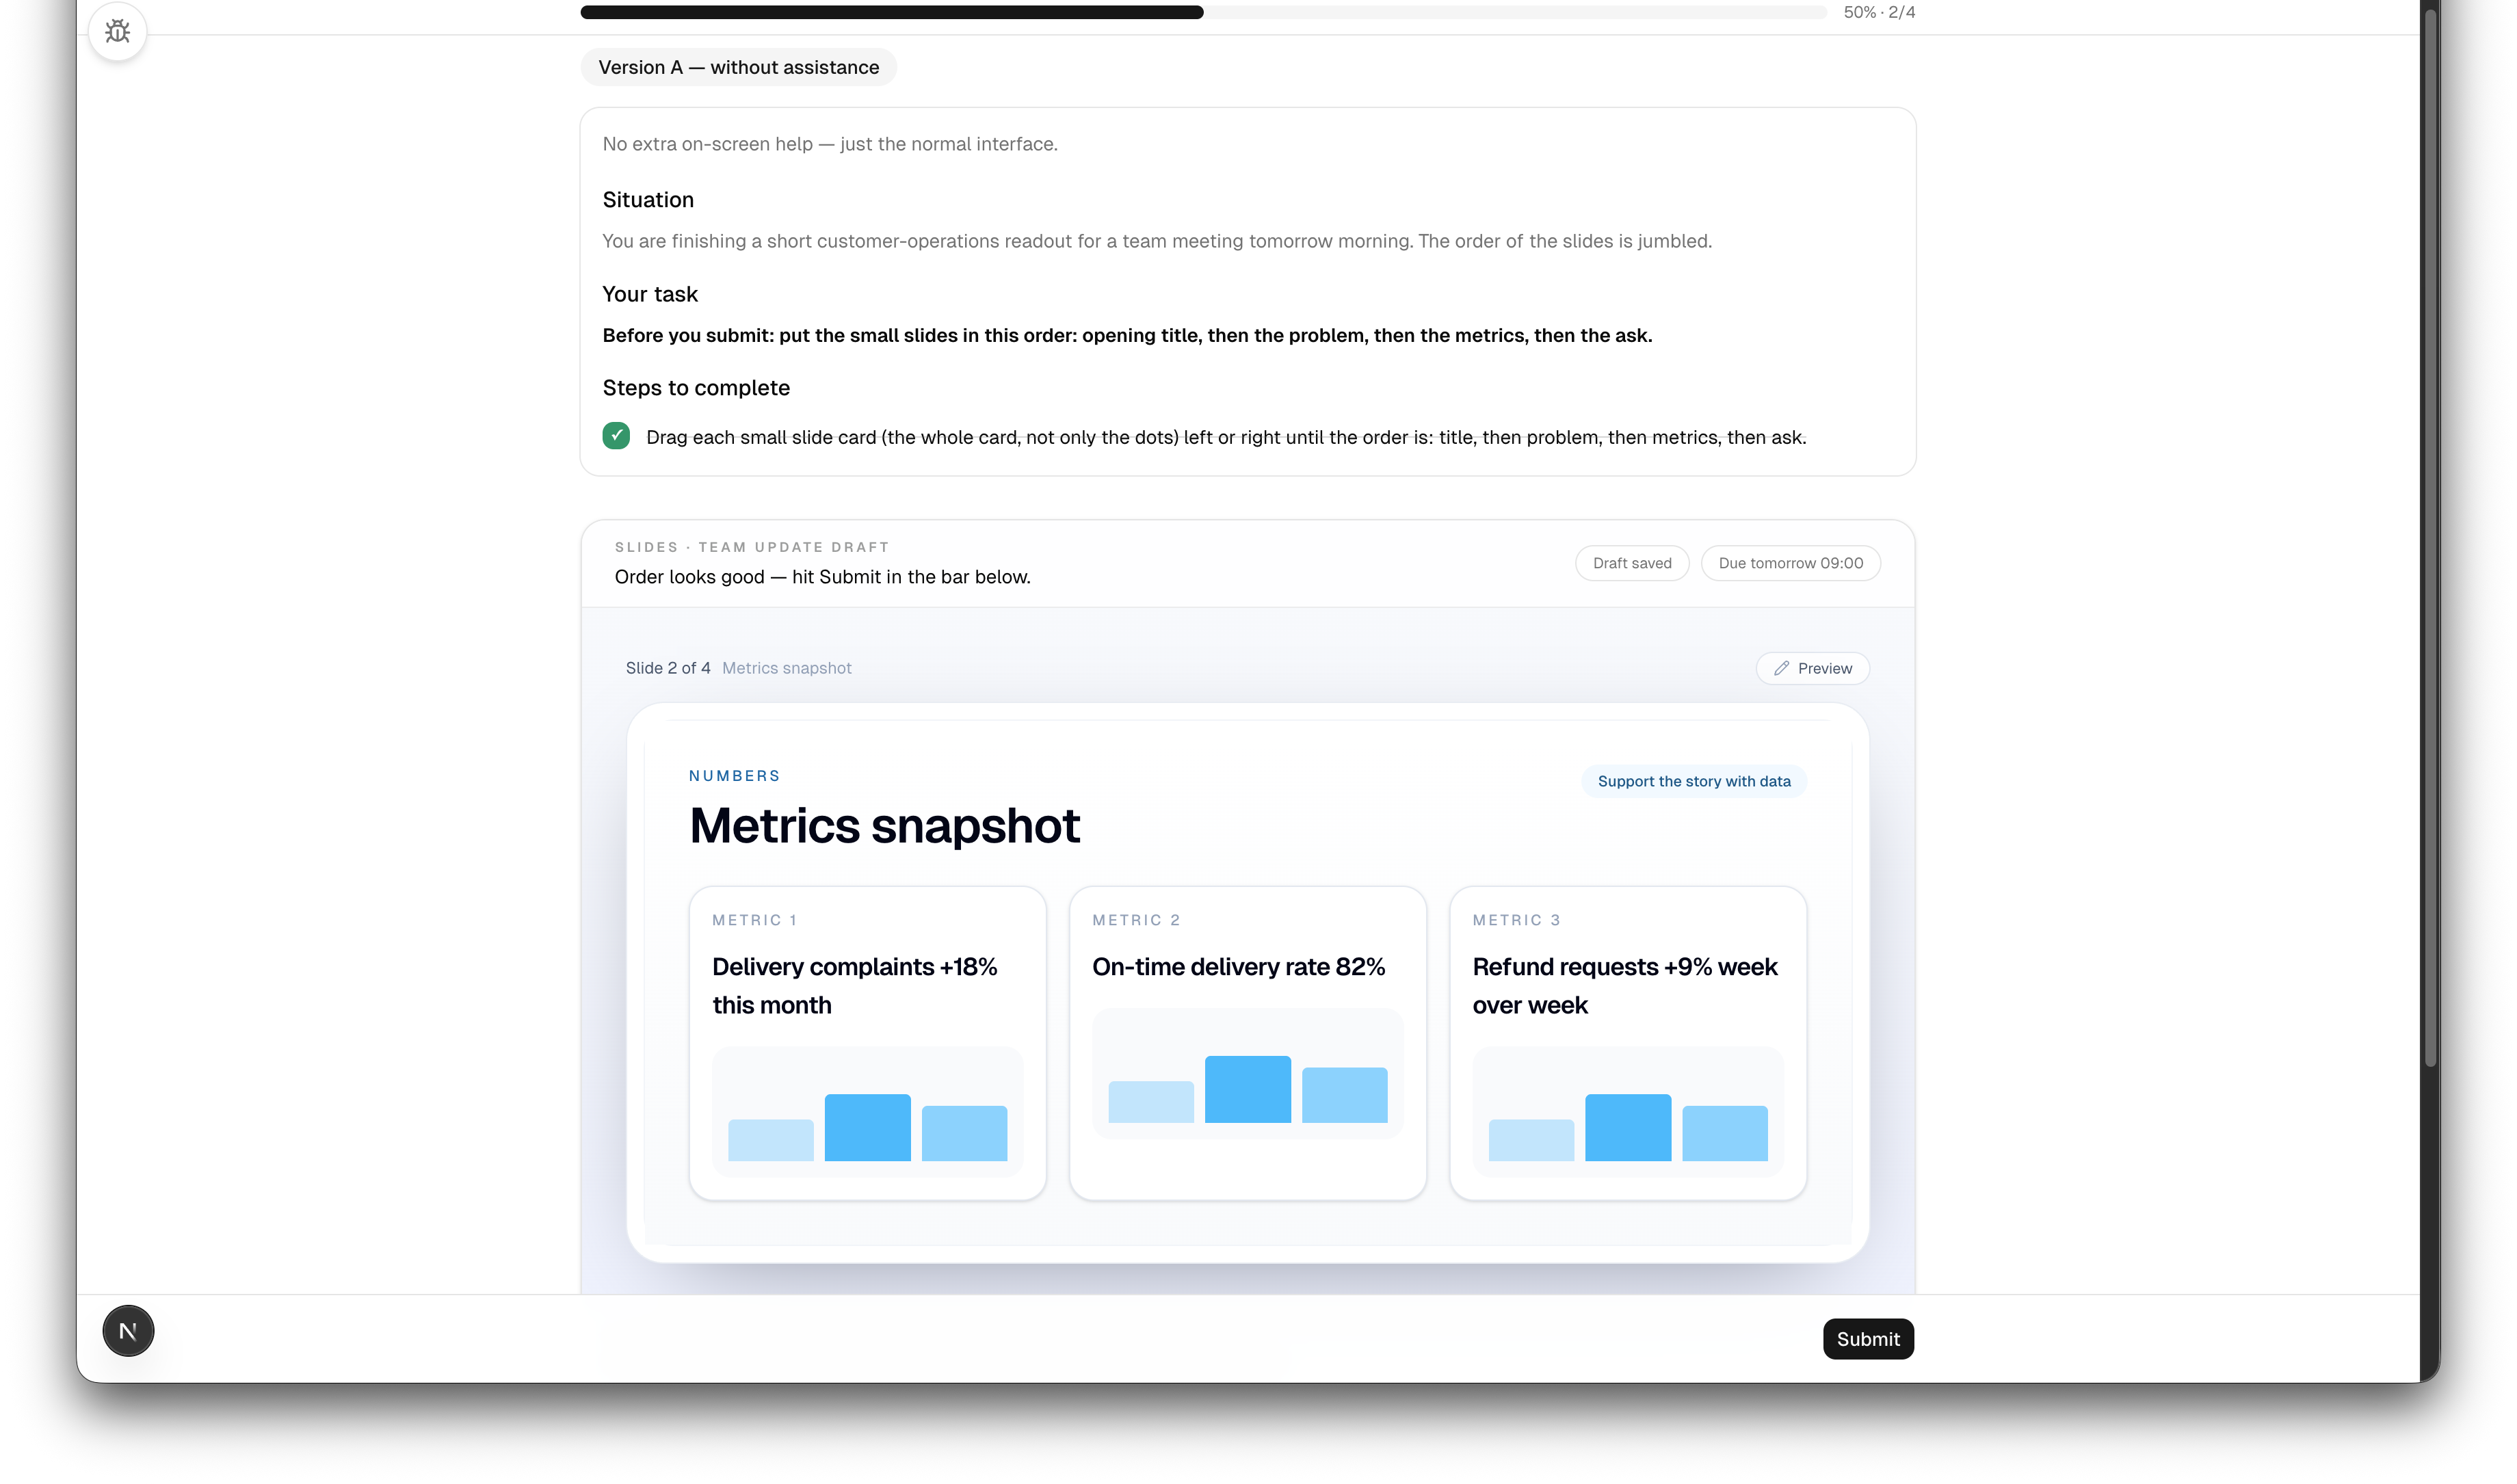
\includegraphics[width=\textwidth]{graphics/example-flow-1.png}
        \caption{Baseline trial with the plain interface visible and no temporary support.}
    \end{subfigure}
    \hfill
    \begin{subfigure}[t]{0.49\textwidth}
        \centering
        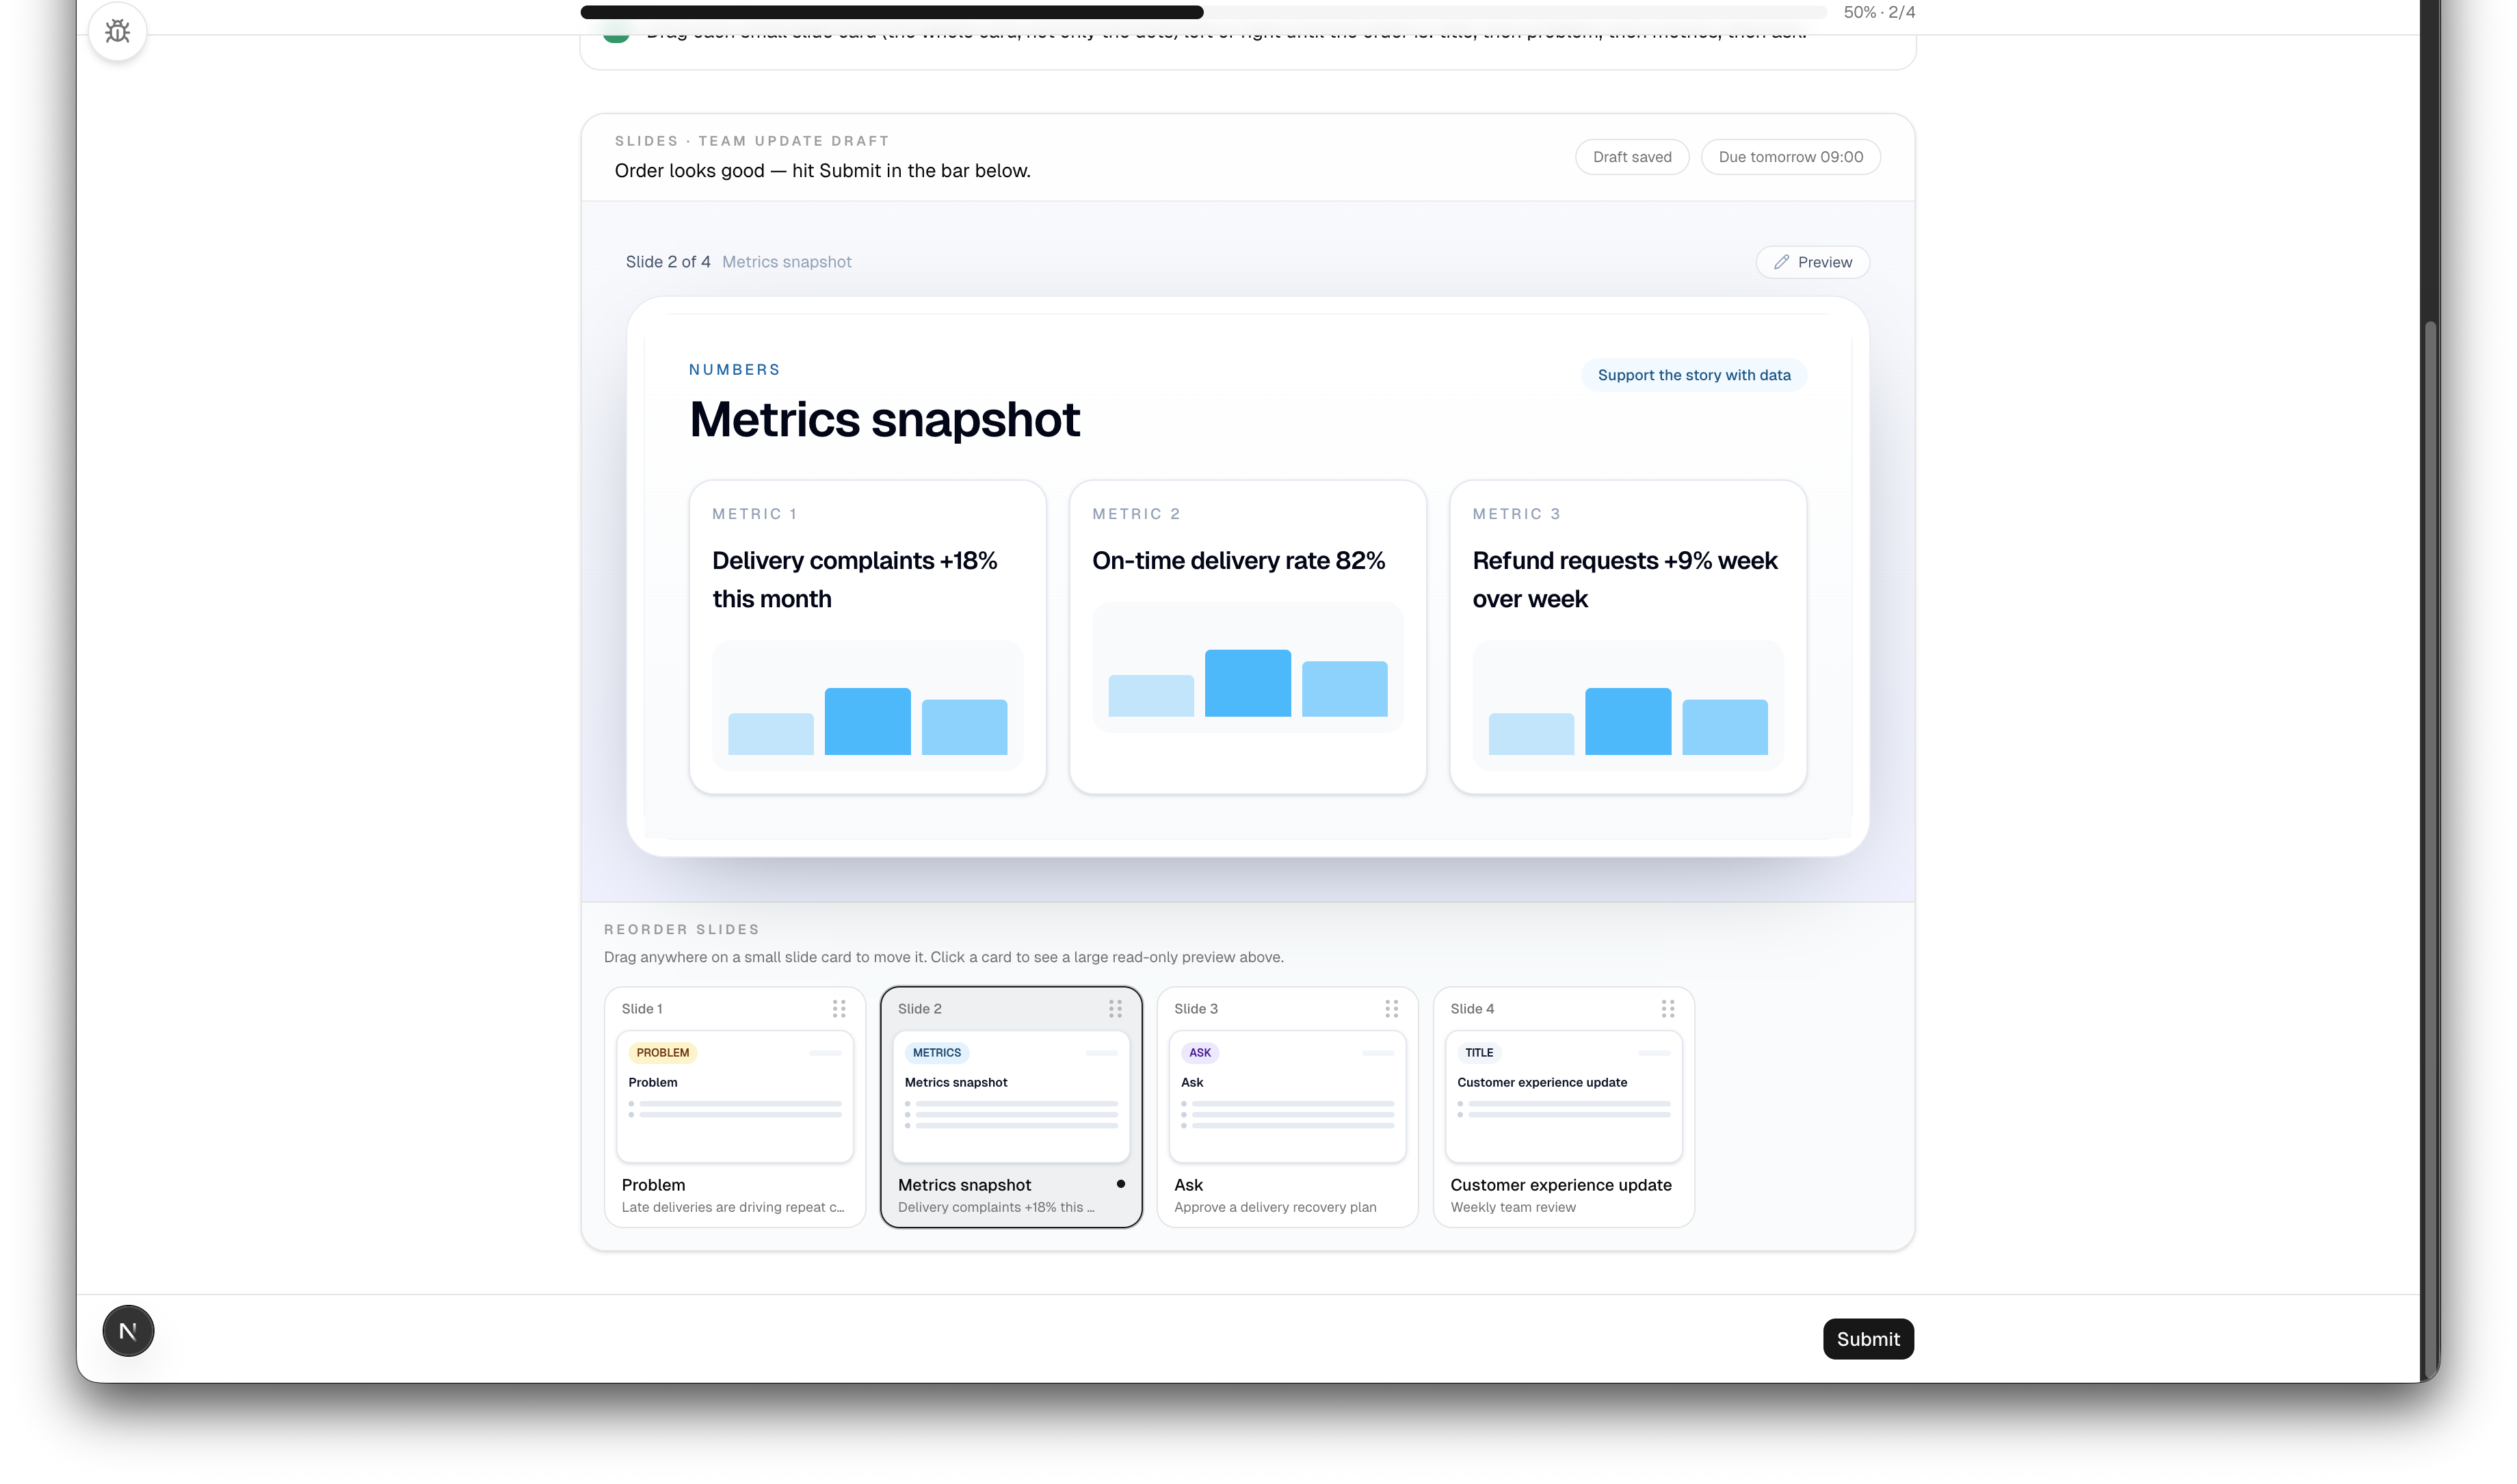
\includegraphics[width=\textwidth]{graphics/example-flow-2.png}
        \caption{Baseline task interaction while the participant reorders the slide strip.}
    \end{subfigure}
    \caption{Participant-flow walkthrough, part~1: baseline-condition task screens.}
    \label{fig:appendix-flow-1}
\end{figure}

\begin{figure}[htbp]
    \centering
    \begin{subfigure}[t]{0.49\textwidth}
        \centering
        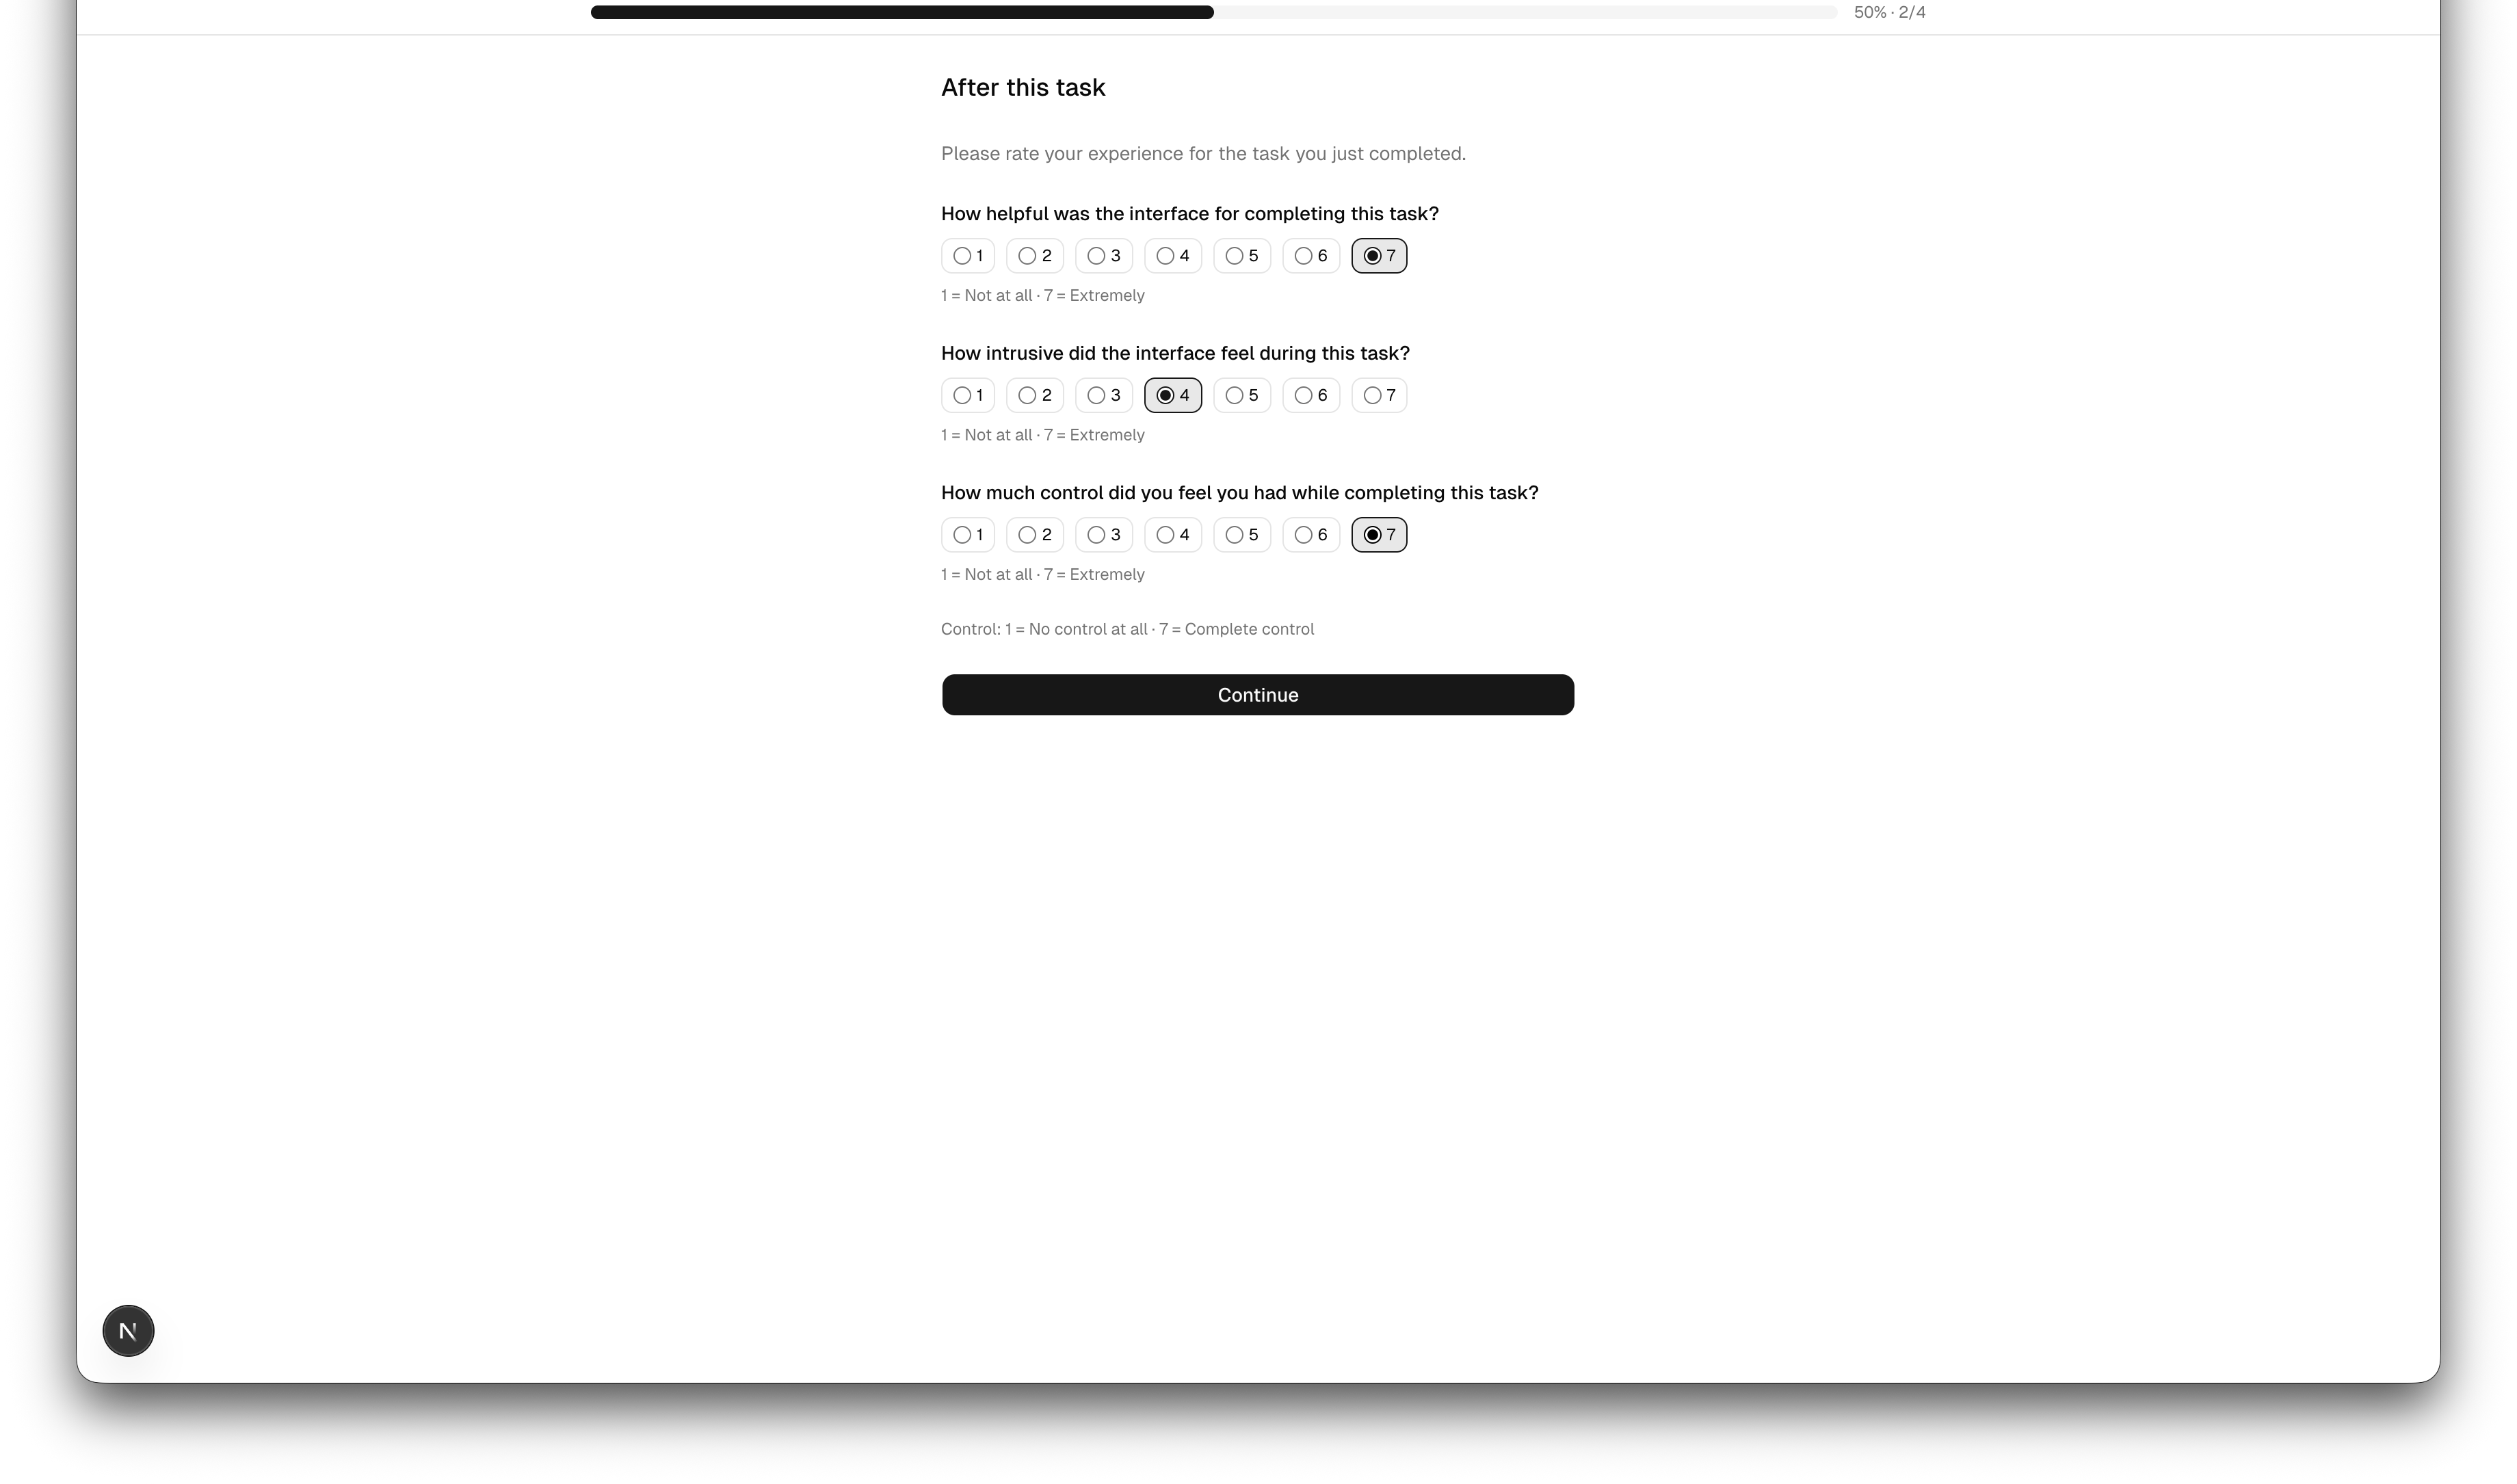
\includegraphics[width=\textwidth]{graphics/example-flow-3.png}
        \caption{Baseline post-trial questionnaire immediately after task completion.}
    \end{subfigure}
    \hfill
    \begin{subfigure}[t]{0.49\textwidth}
        \centering
        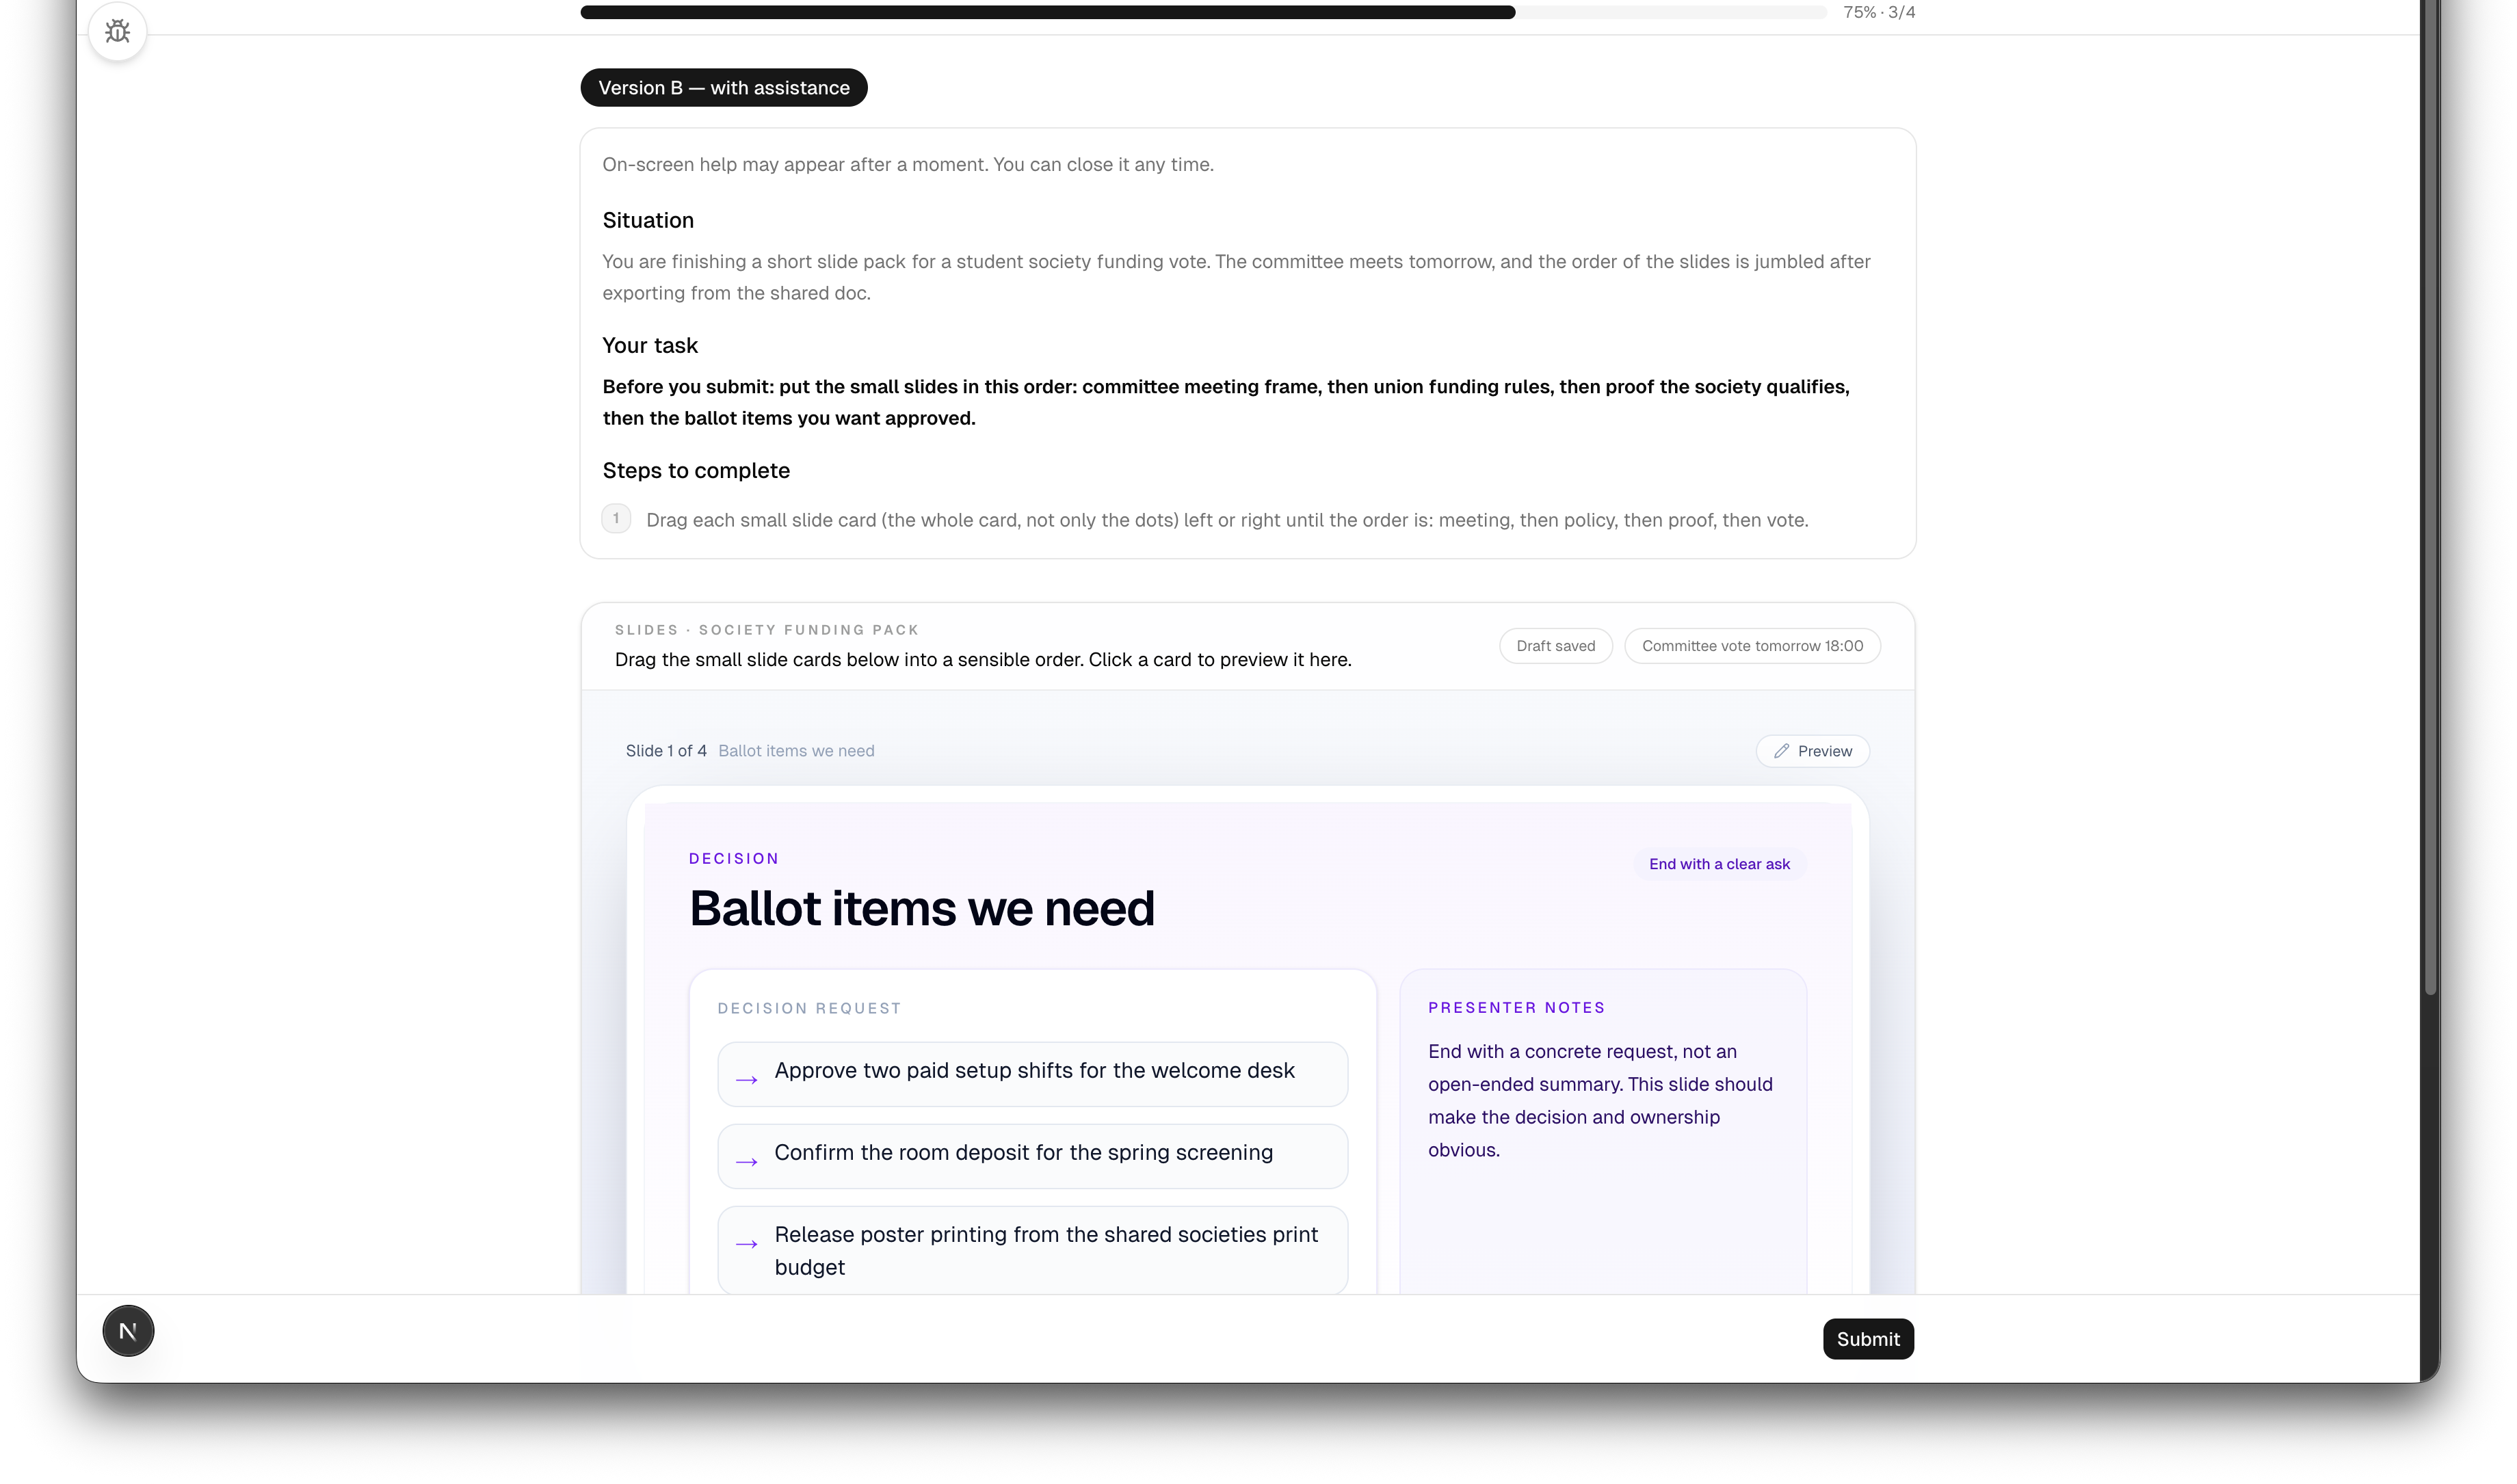
\includegraphics[width=\textwidth]{graphics/example-flow-4.png}
        \caption{Start of the ephemeral-condition trial, which warns that temporary help may appear.}
    \end{subfigure}
    \caption{Participant-flow walkthrough, part~2: transition from the baseline trial to the ephemeral trial.}
    \label{fig:appendix-flow-2}
\end{figure}

\begin{figure}[htbp]
    \centering
    \begin{subfigure}[t]{0.49\textwidth}
        \centering
        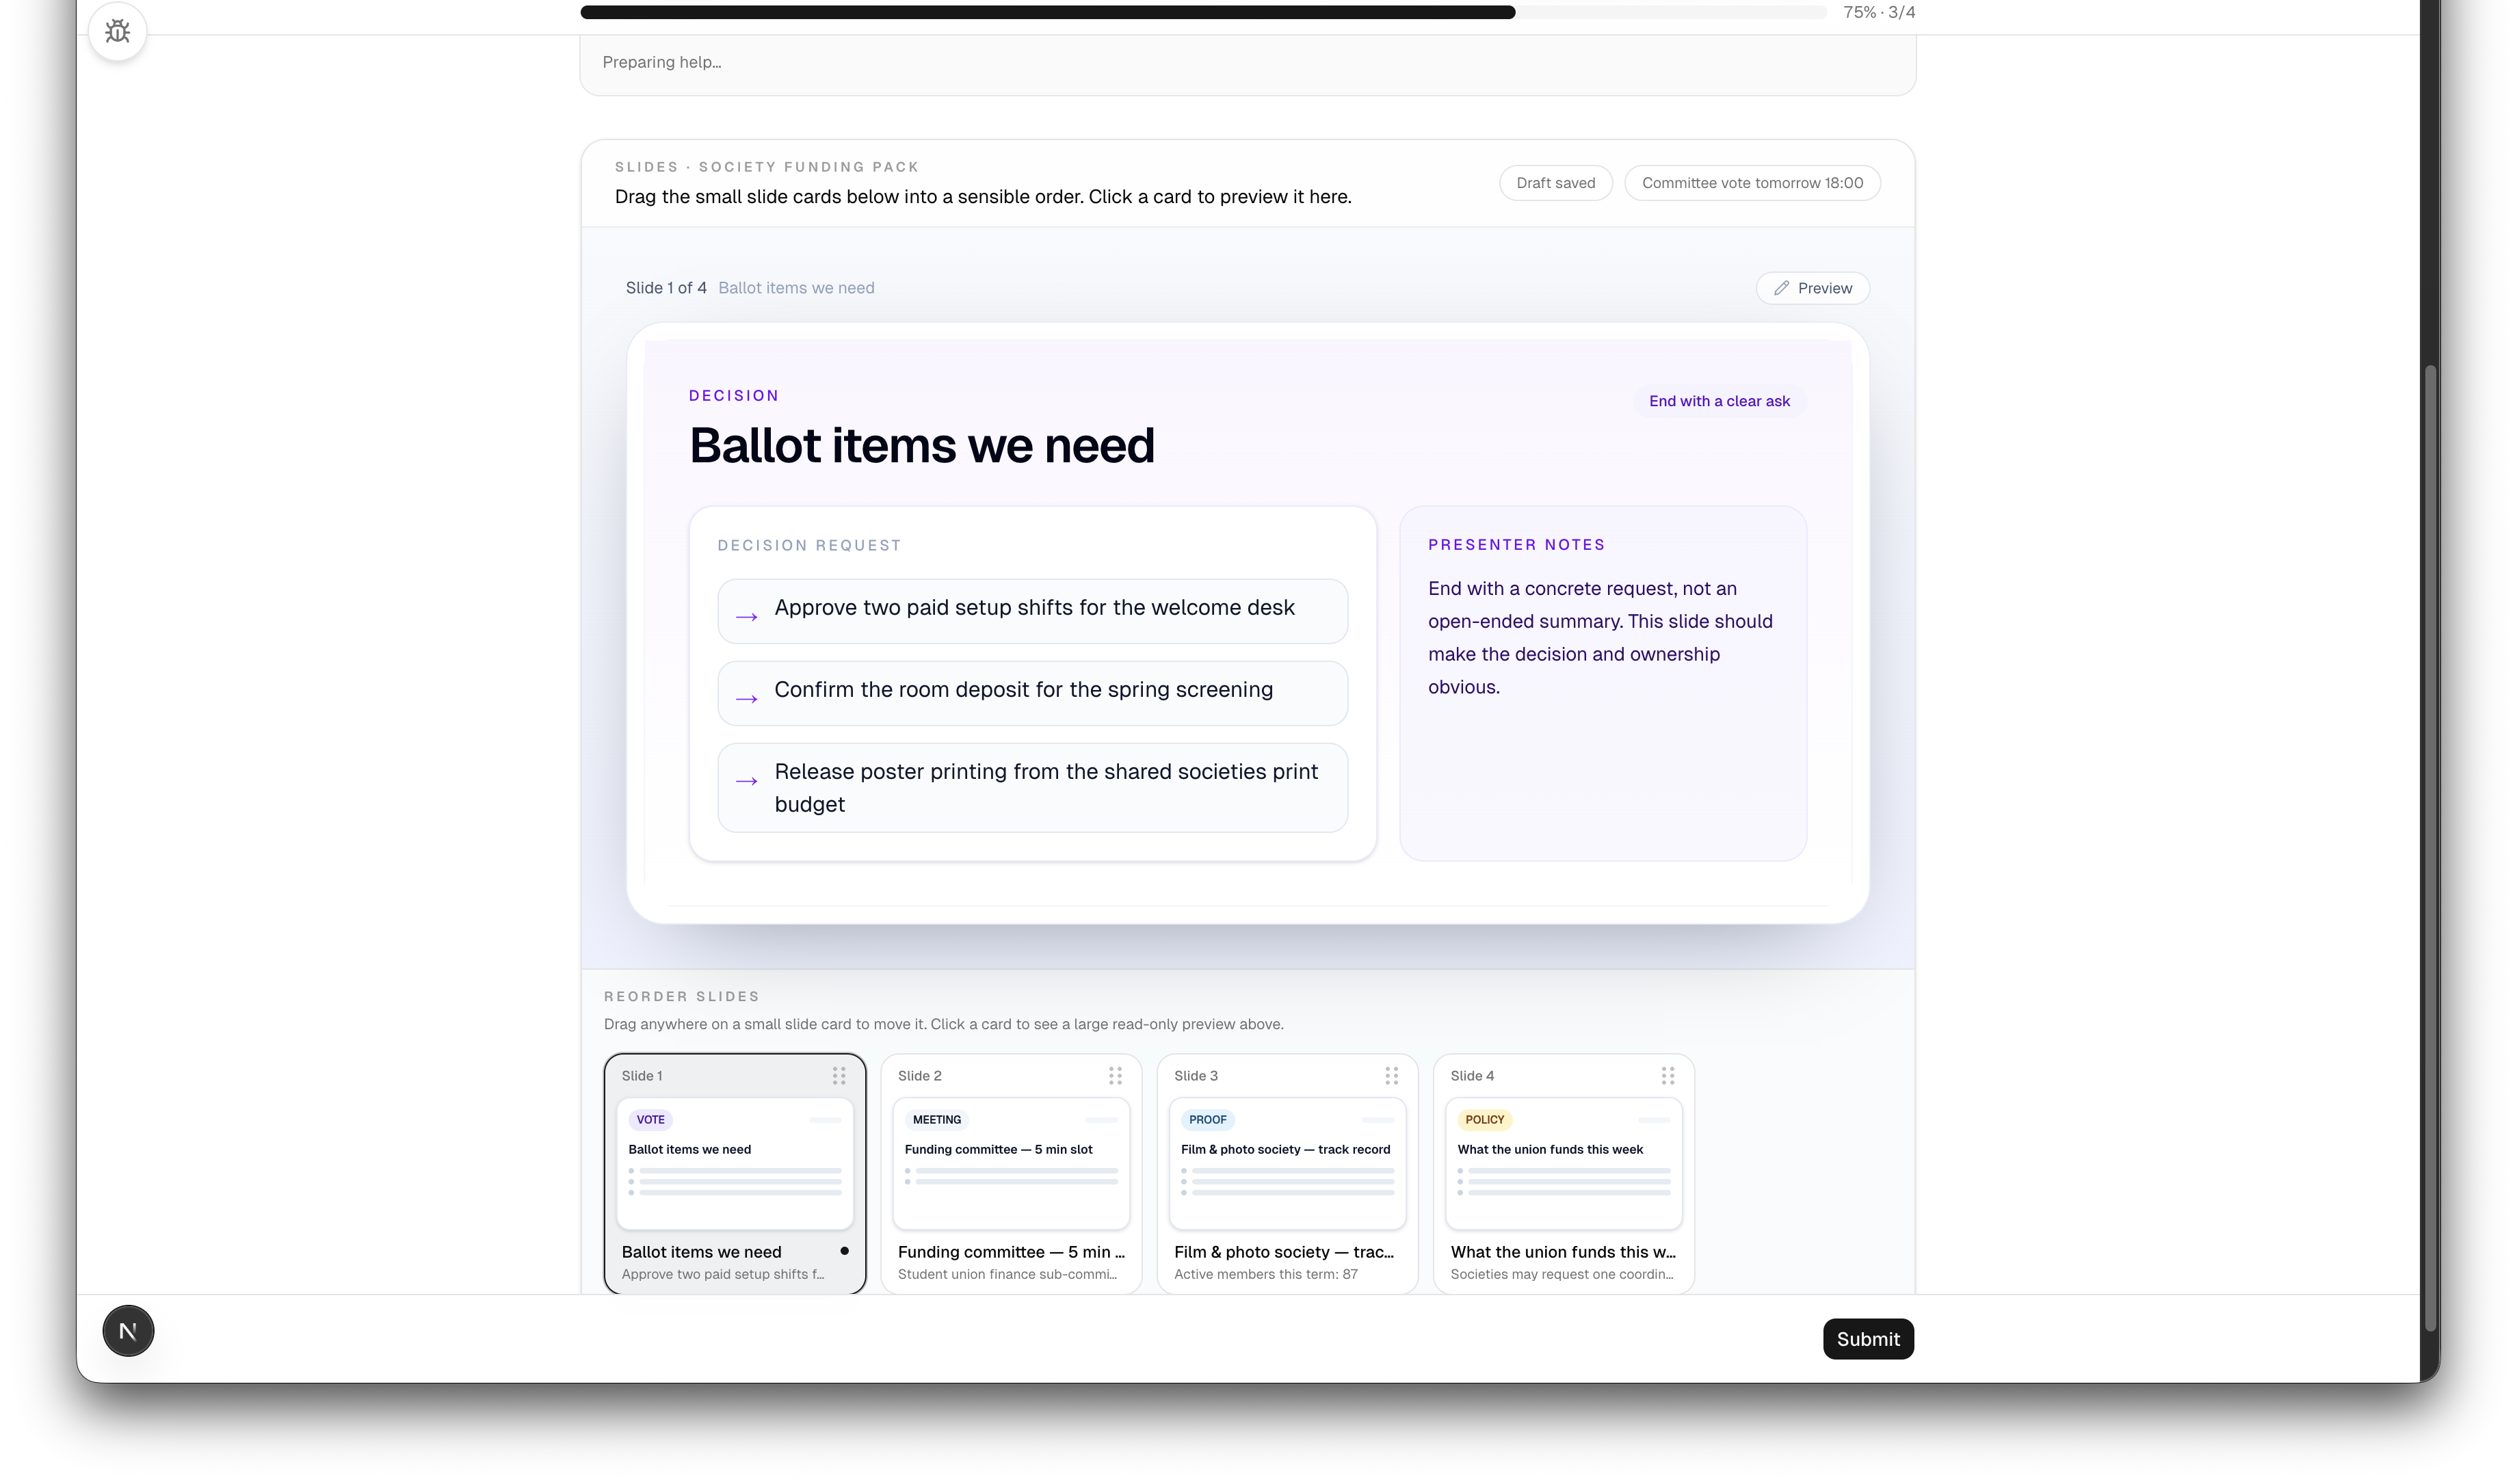
\includegraphics[width=\textwidth]{graphics/example-flow-5.png}
        \caption{Ephemeral-condition task before the support overlay expands.}
    \end{subfigure}
    \hfill
    \begin{subfigure}[t]{0.49\textwidth}
        \centering
        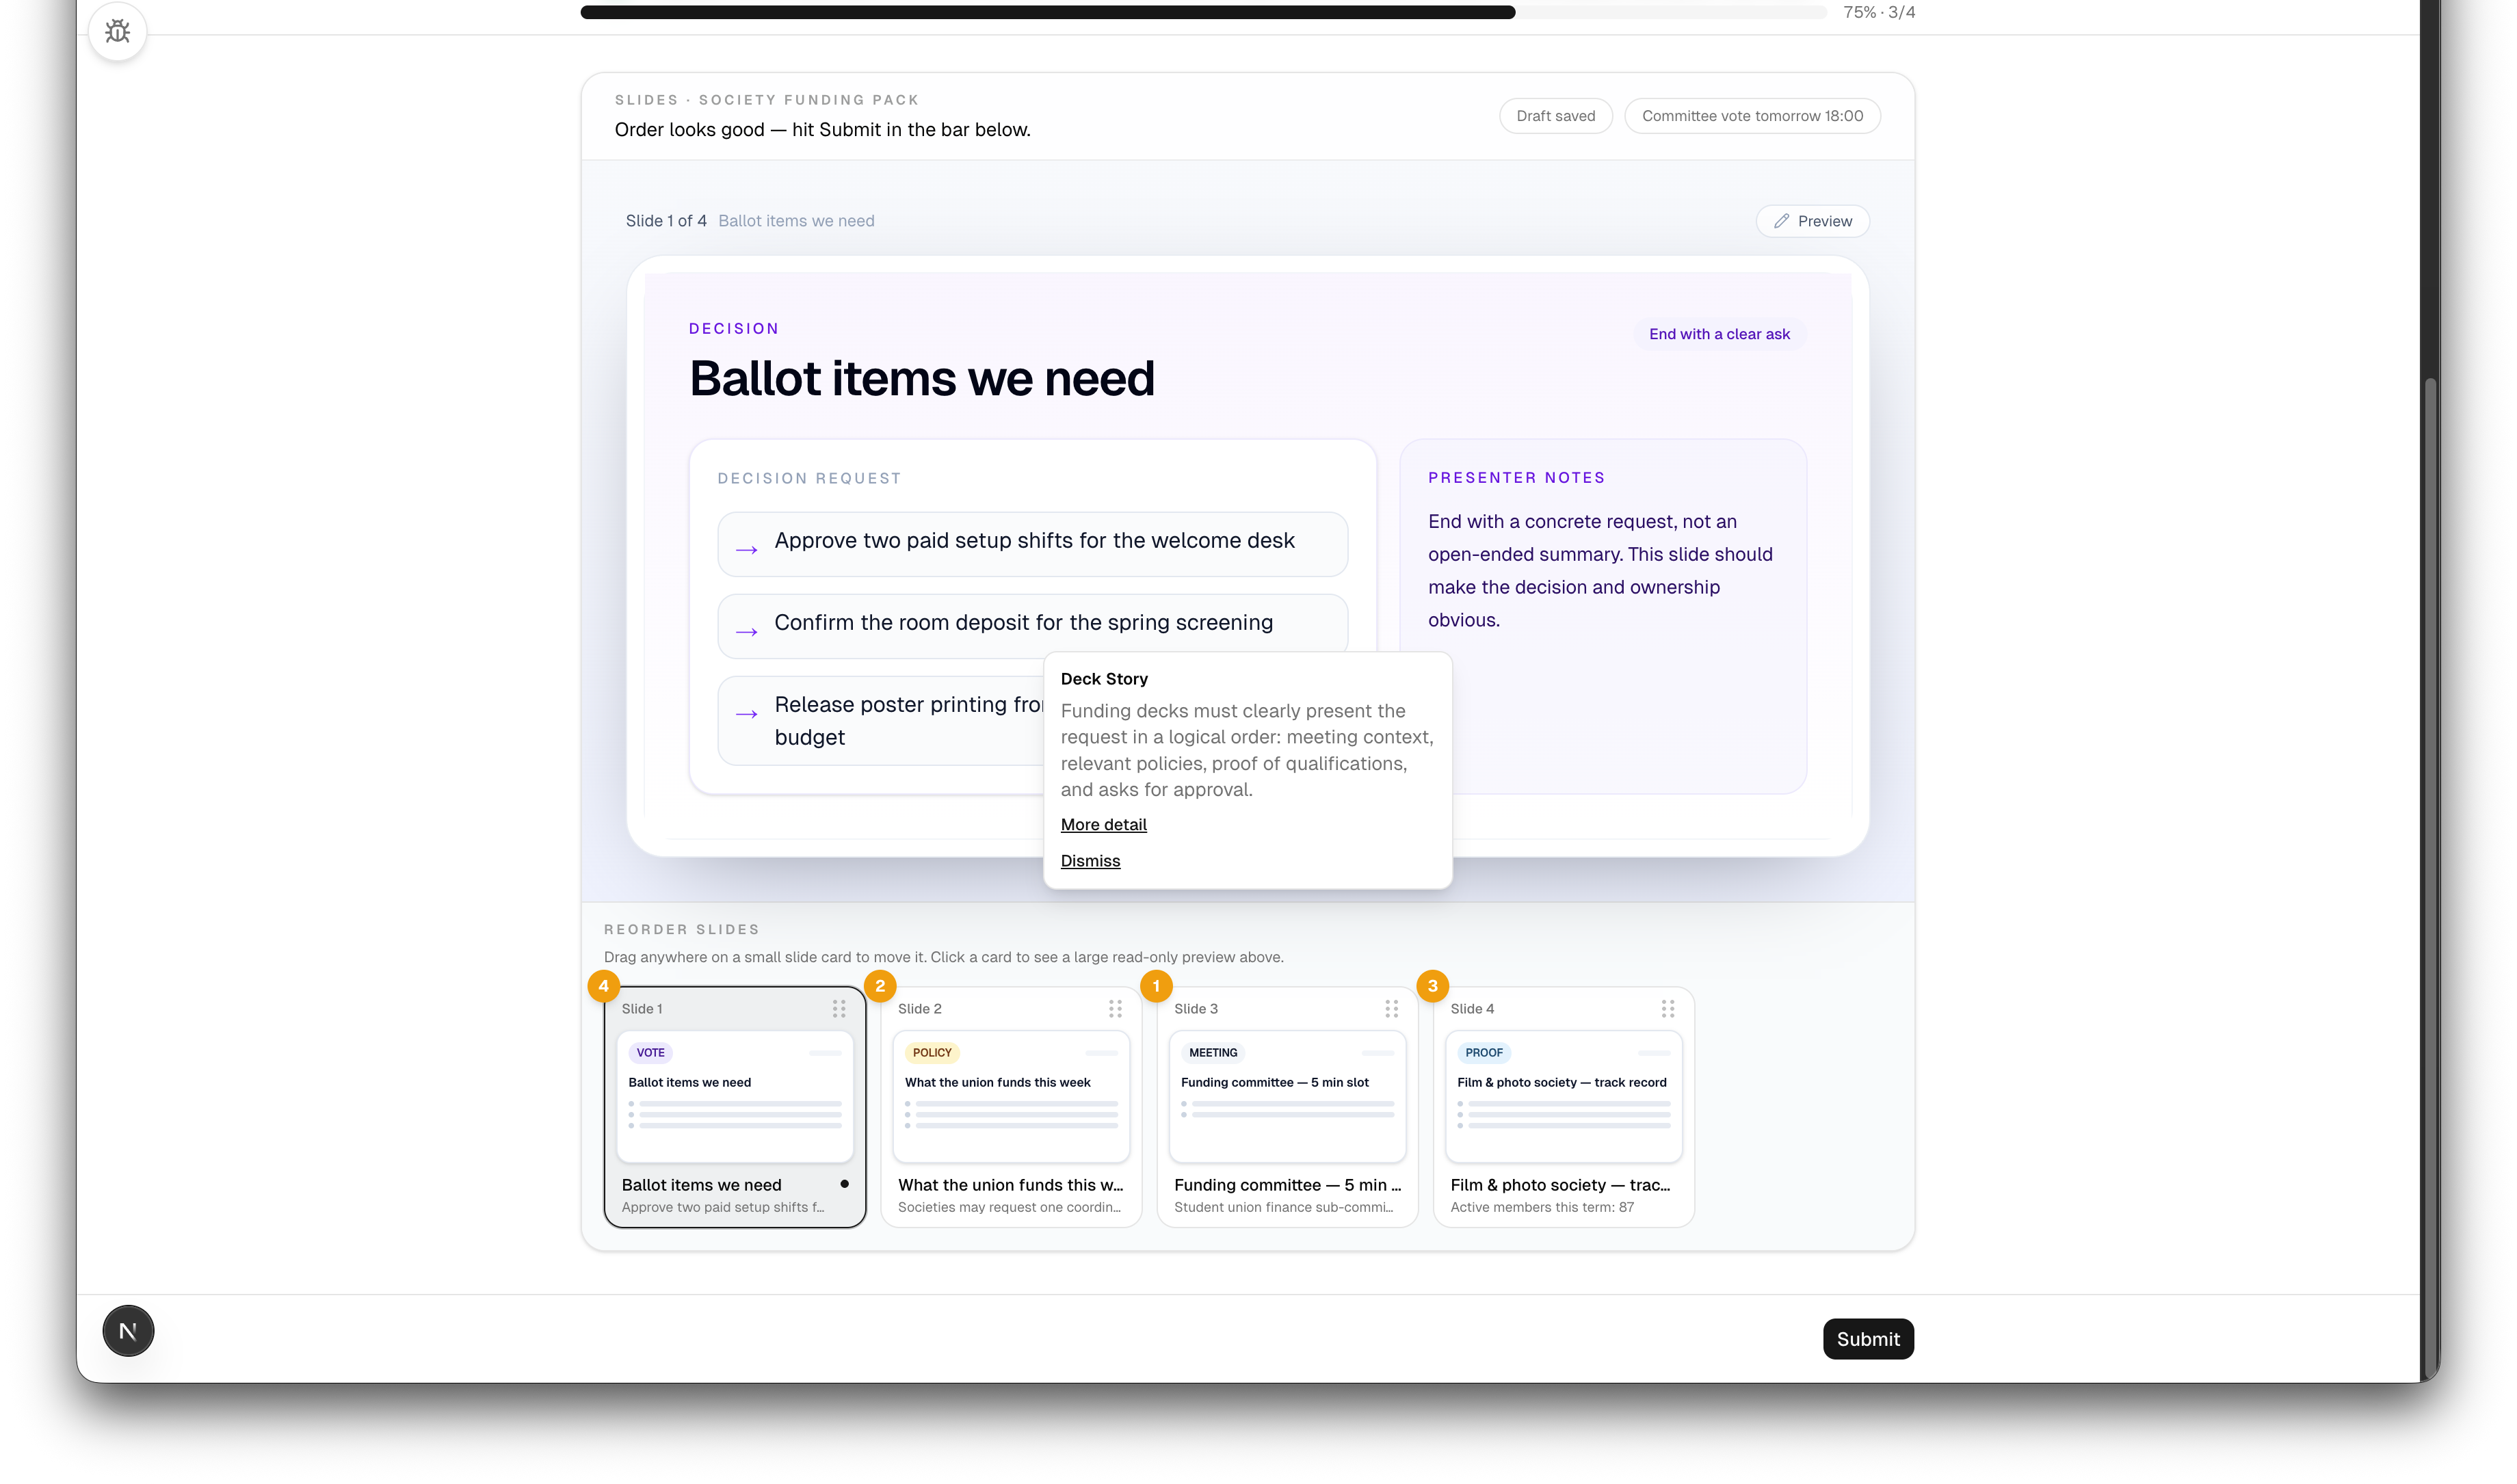
\includegraphics[width=\textwidth]{graphics/example-flow-6.png}
        \caption{Generated support visible as an anchored explanation and ordered markers over the slide strip.}
    \end{subfigure}
    \caption{Participant-flow walkthrough, part~3: ephemeral assistance becoming visible during the task.}
    \label{fig:appendix-flow-3}
\end{figure}

\begin{figure}[htbp]
    \centering
    \begin{subfigure}[t]{0.49\textwidth}
        \centering
        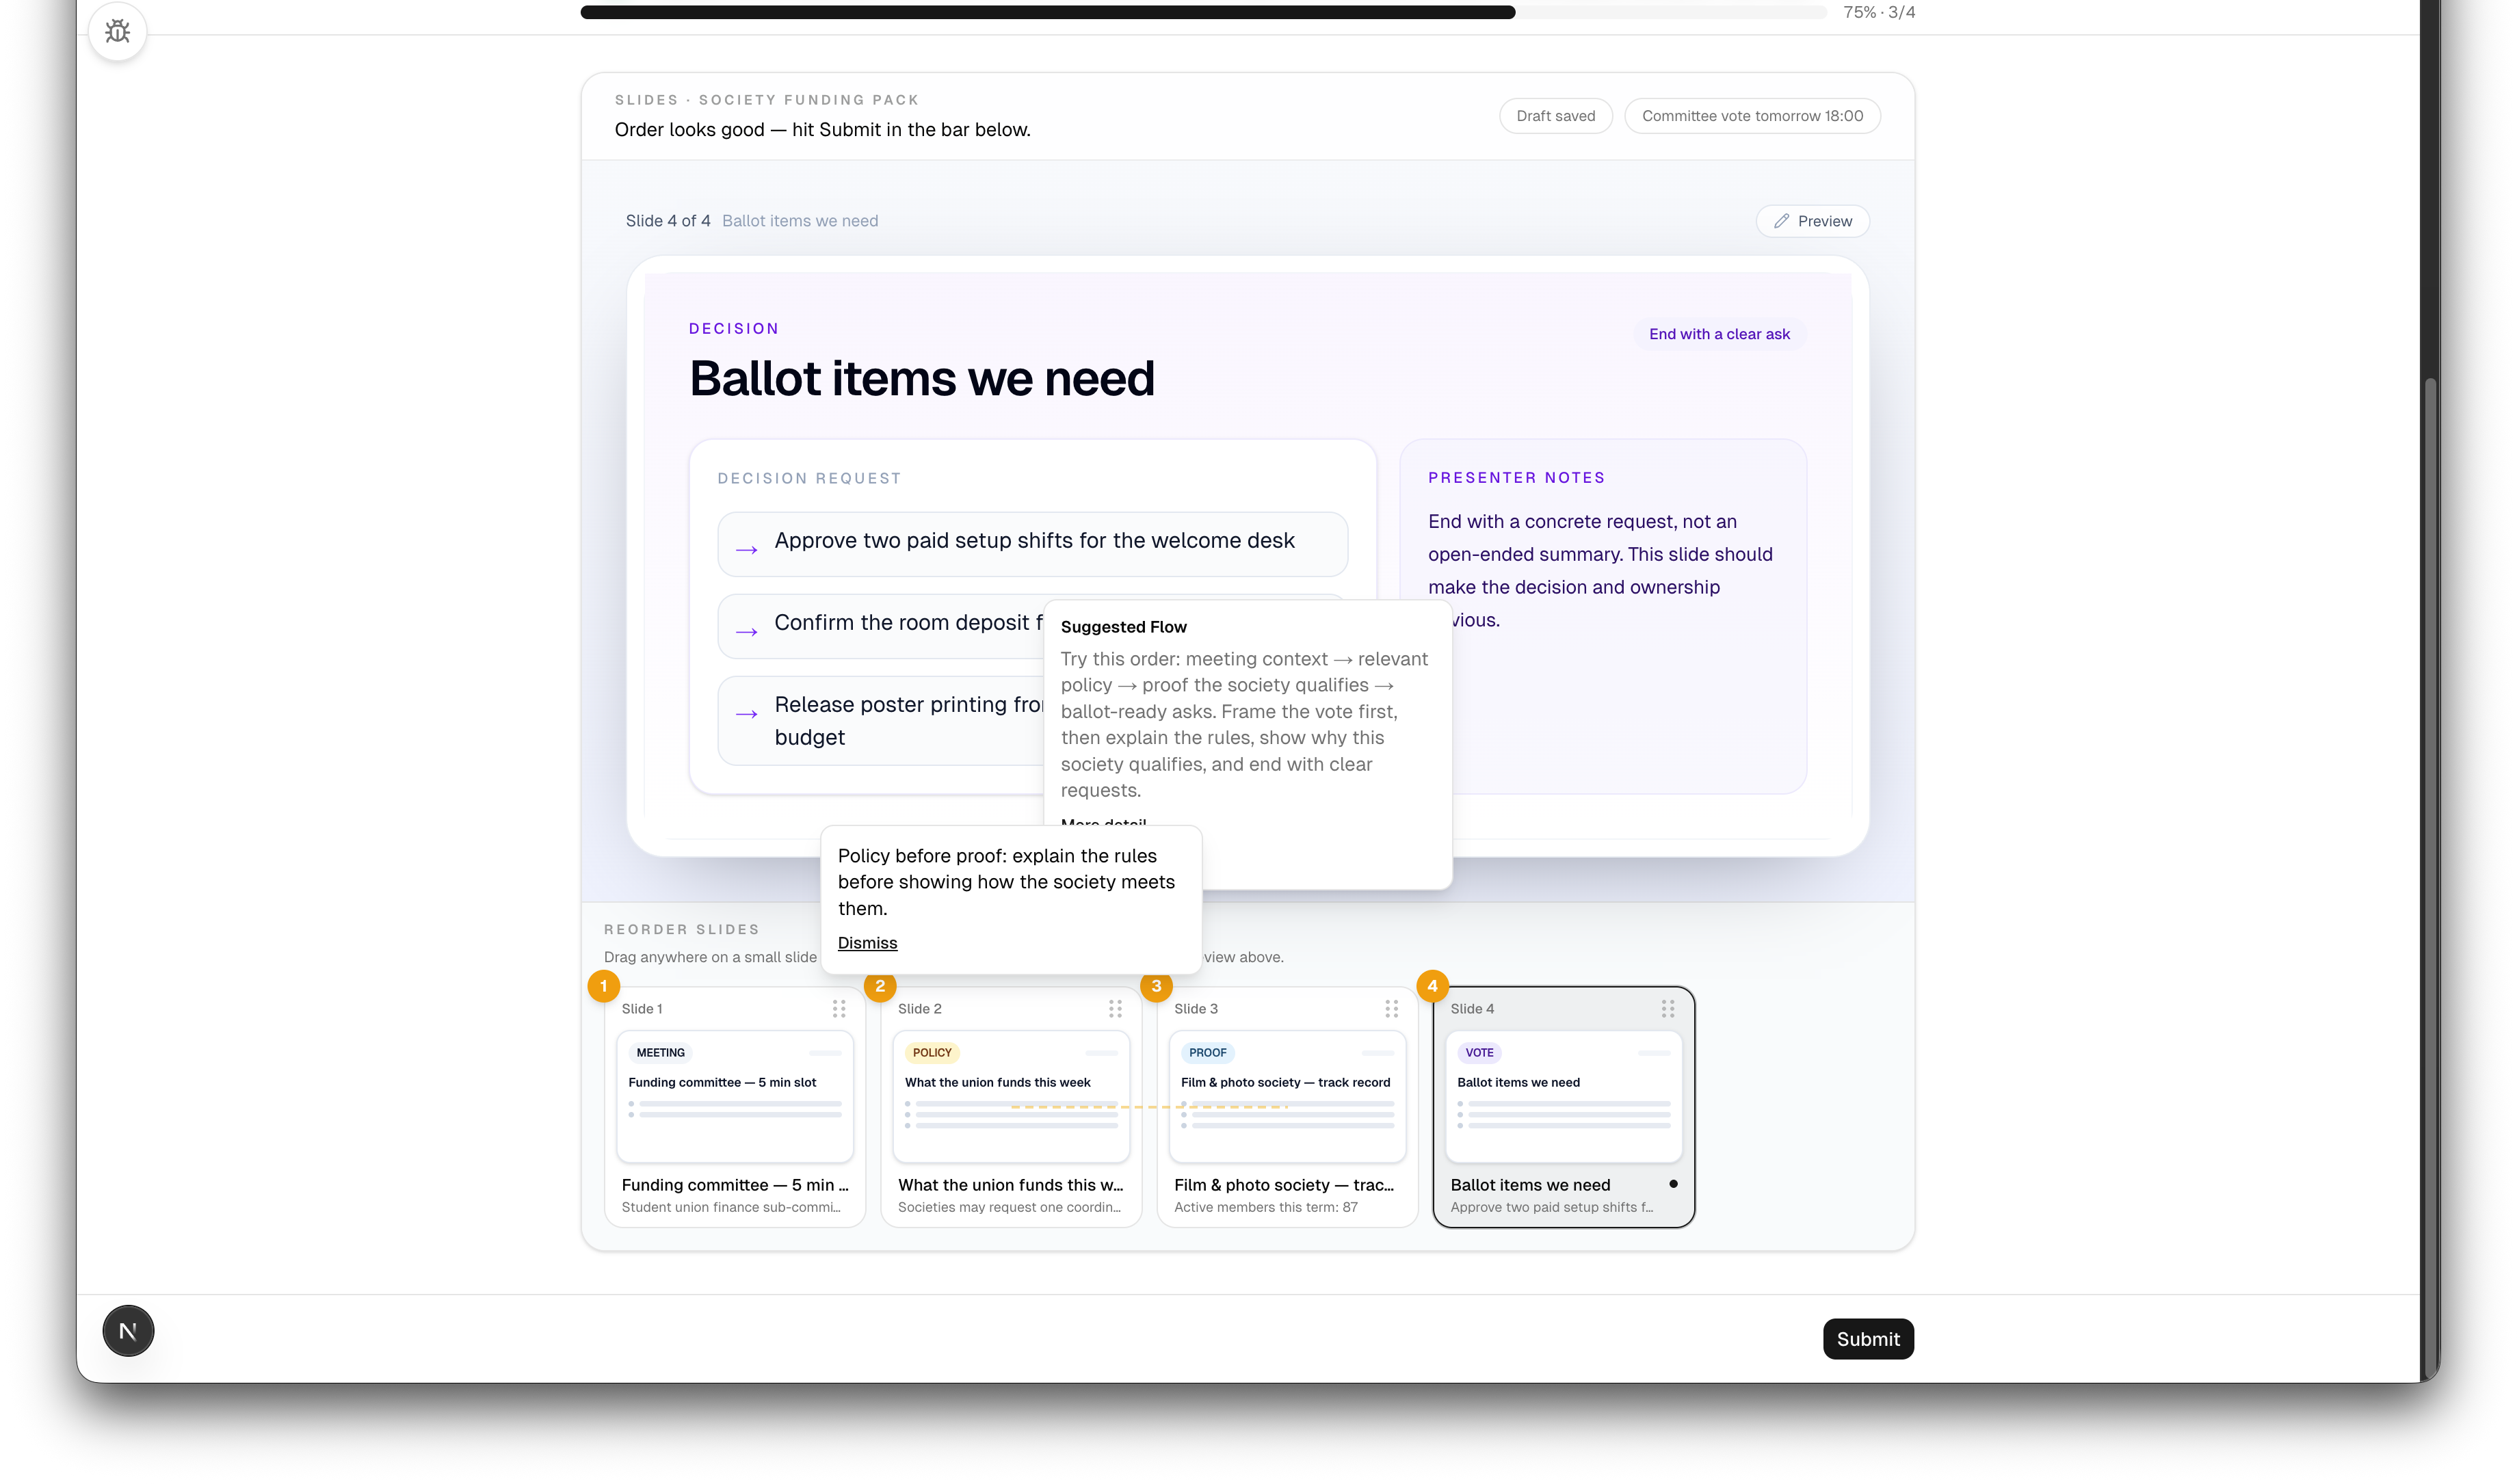
\includegraphics[width=\textwidth]{graphics/example-flow-7.png}
        \caption{Ephemeral overlay aligned to the current slide and reorder strip.}
    \end{subfigure}
    \hfill
    \begin{subfigure}[t]{0.49\textwidth}
        \centering
        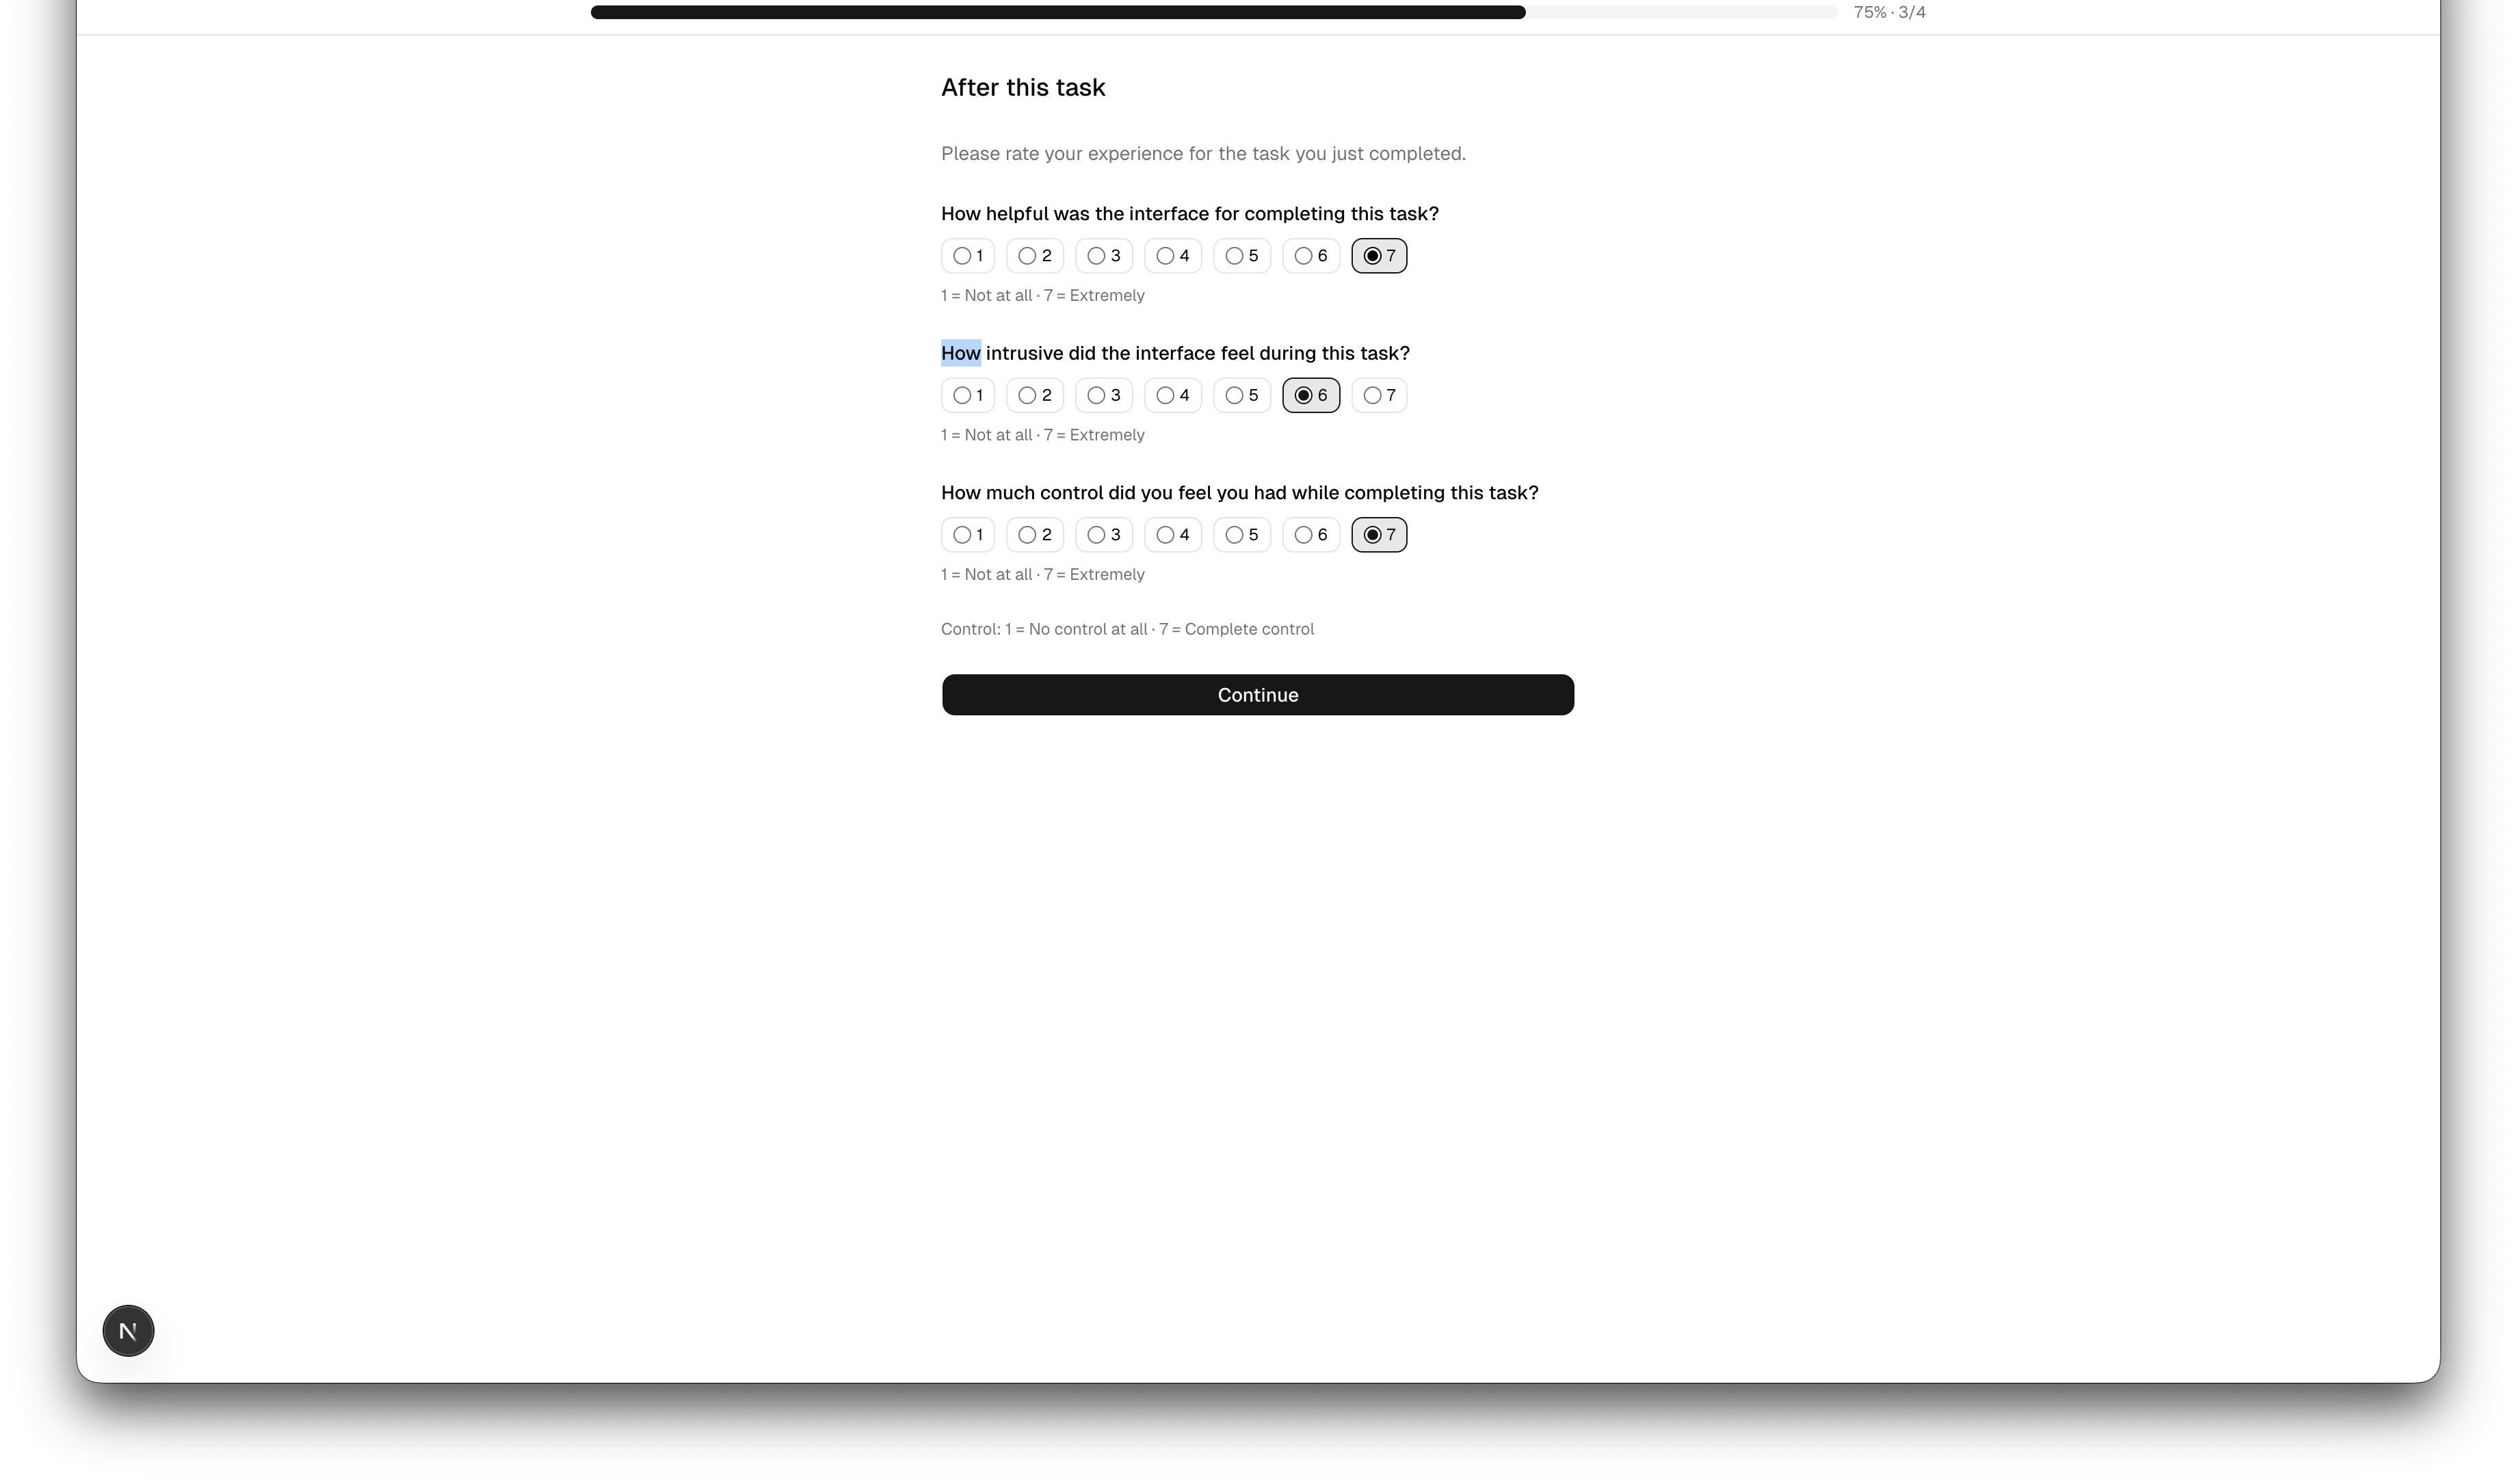
\includegraphics[width=\textwidth]{graphics/example-flow-8.png}
        \caption{Expanded support details combining an inspect panel, tooltip, and ordering cues.}
    \end{subfigure}
    \caption{Participant-flow walkthrough, part~4: richer support states within the ephemeral trial.}
    \label{fig:appendix-flow-4}
\end{figure}

\begin{figure}[htbp]
    \centering
    \begin{subfigure}[t]{0.49\textwidth}
        \centering
        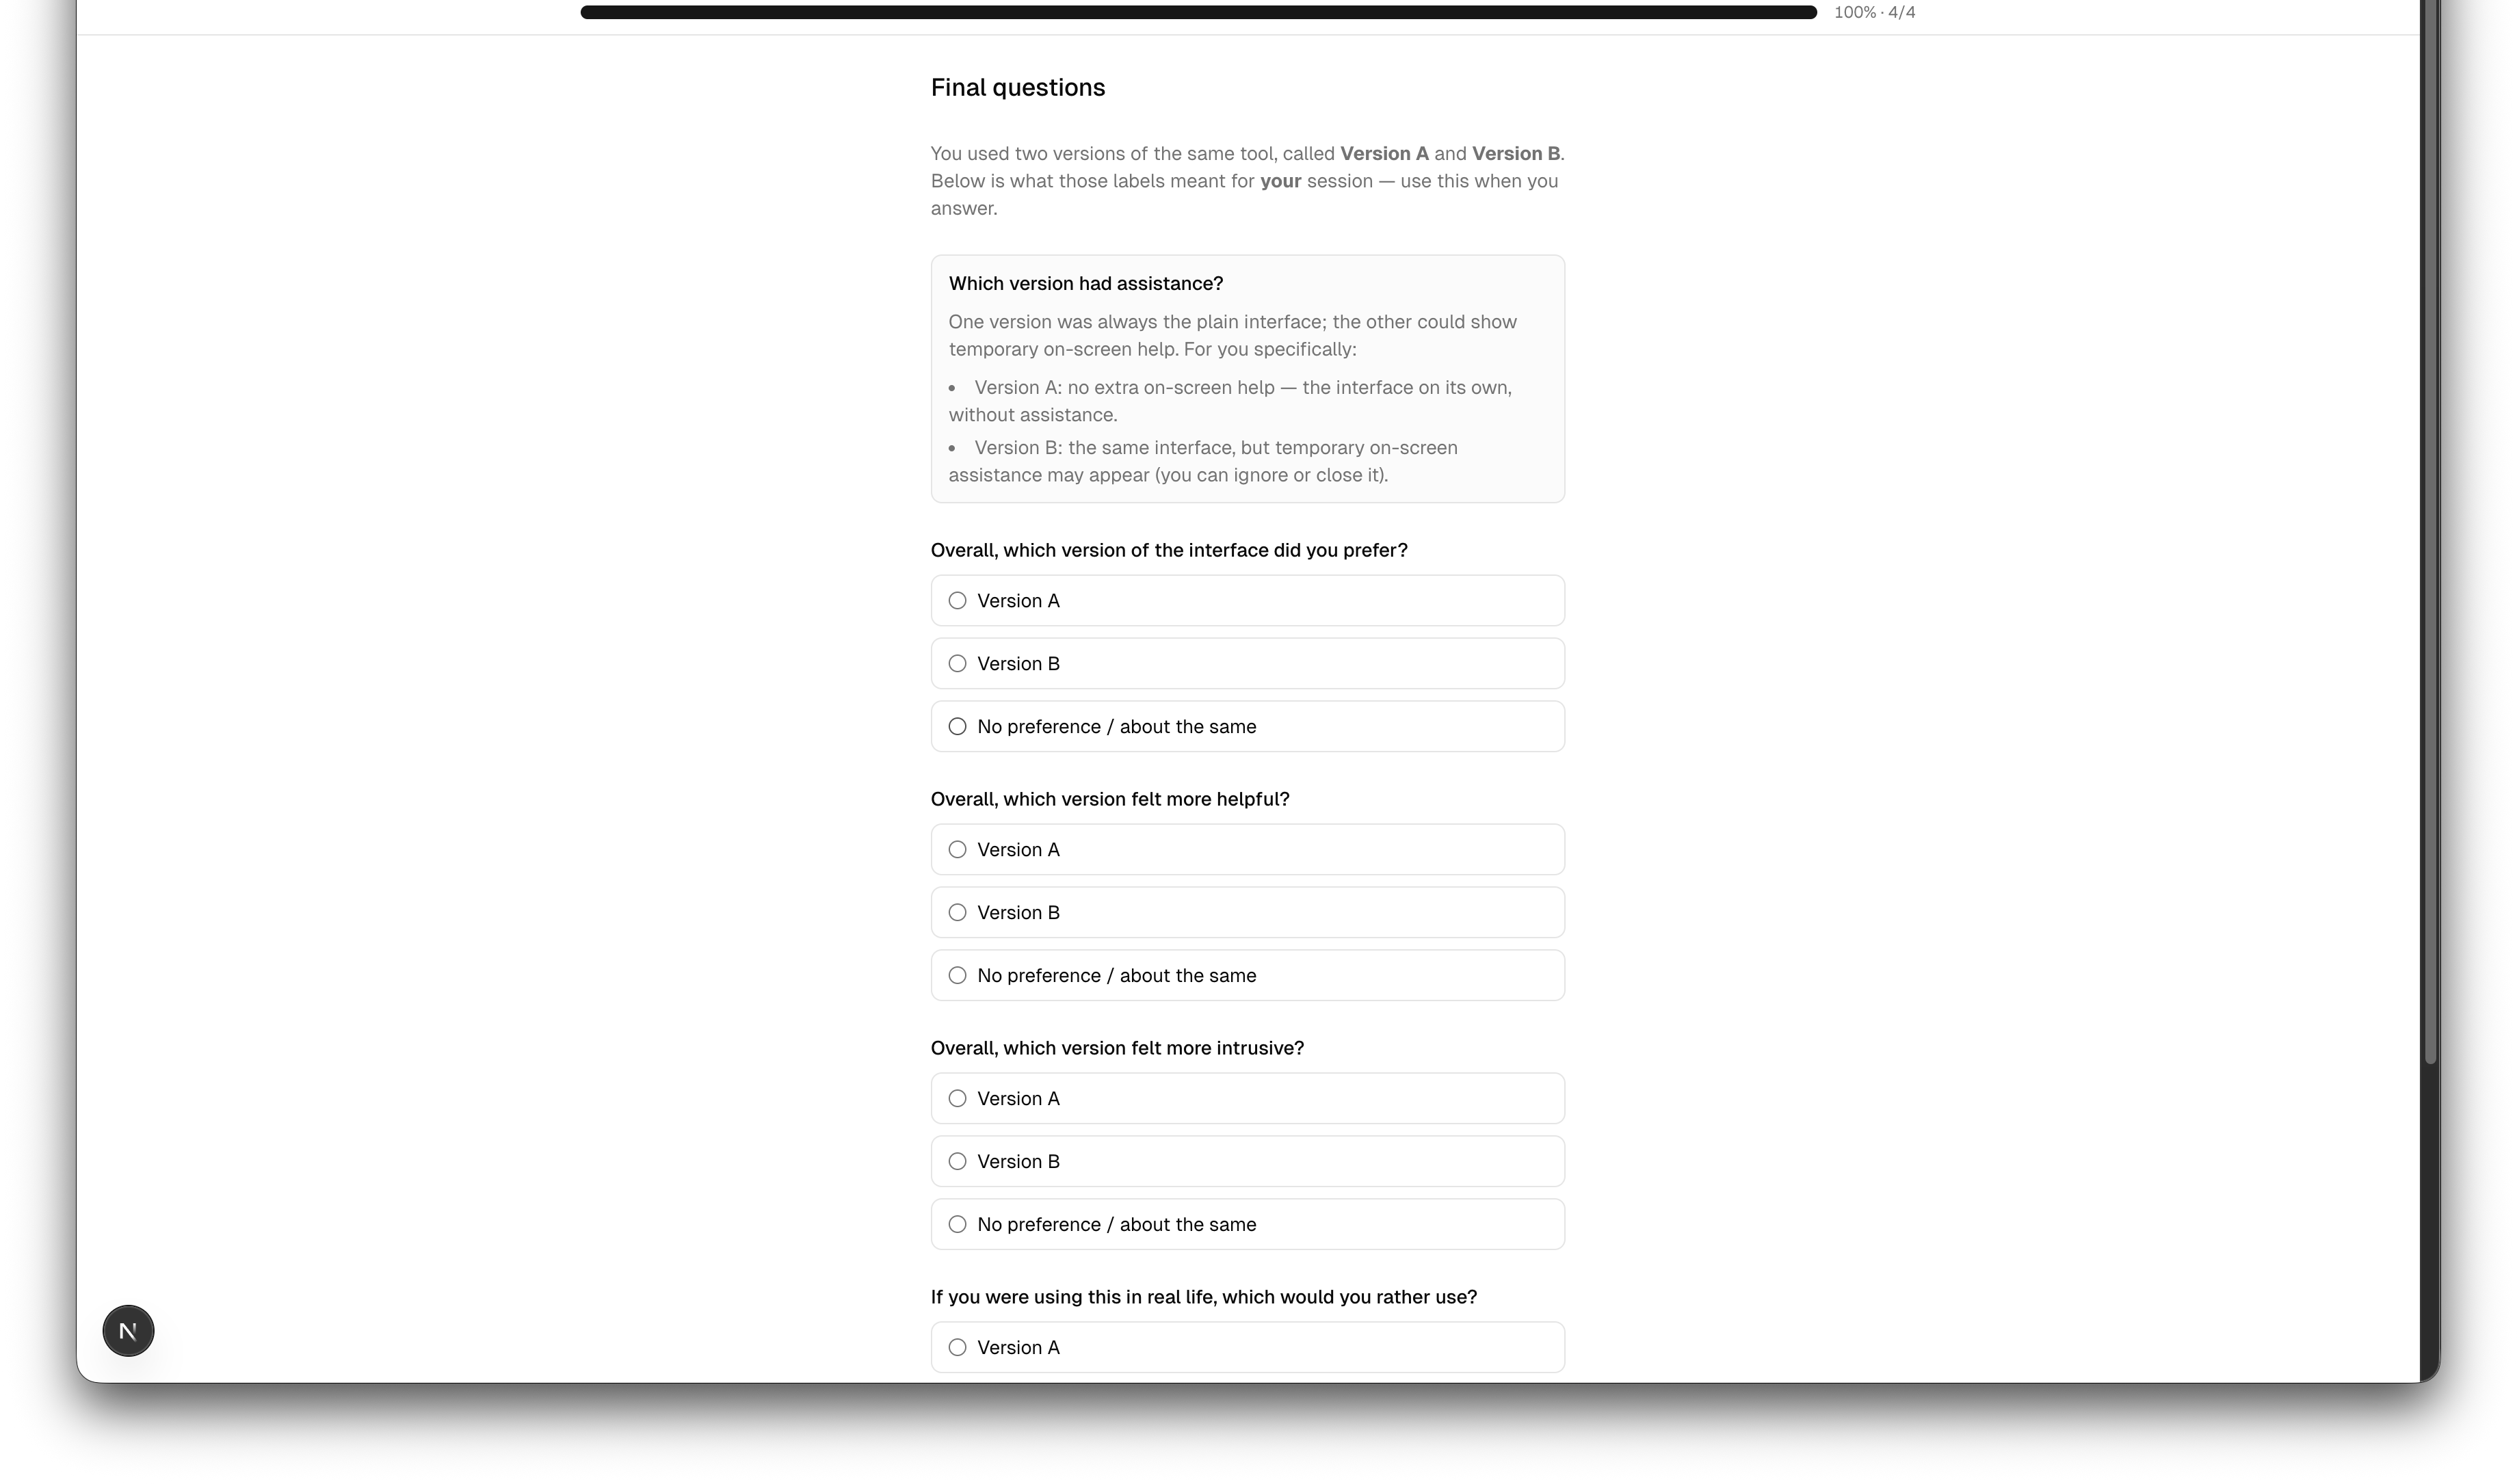
\includegraphics[width=\textwidth]{graphics/example-flow-9.png}
        \caption{Beginning of the final comparative questionnaire after both trials are complete.}
    \end{subfigure}
    \hfill
    \begin{subfigure}[t]{0.49\textwidth}
        \centering
        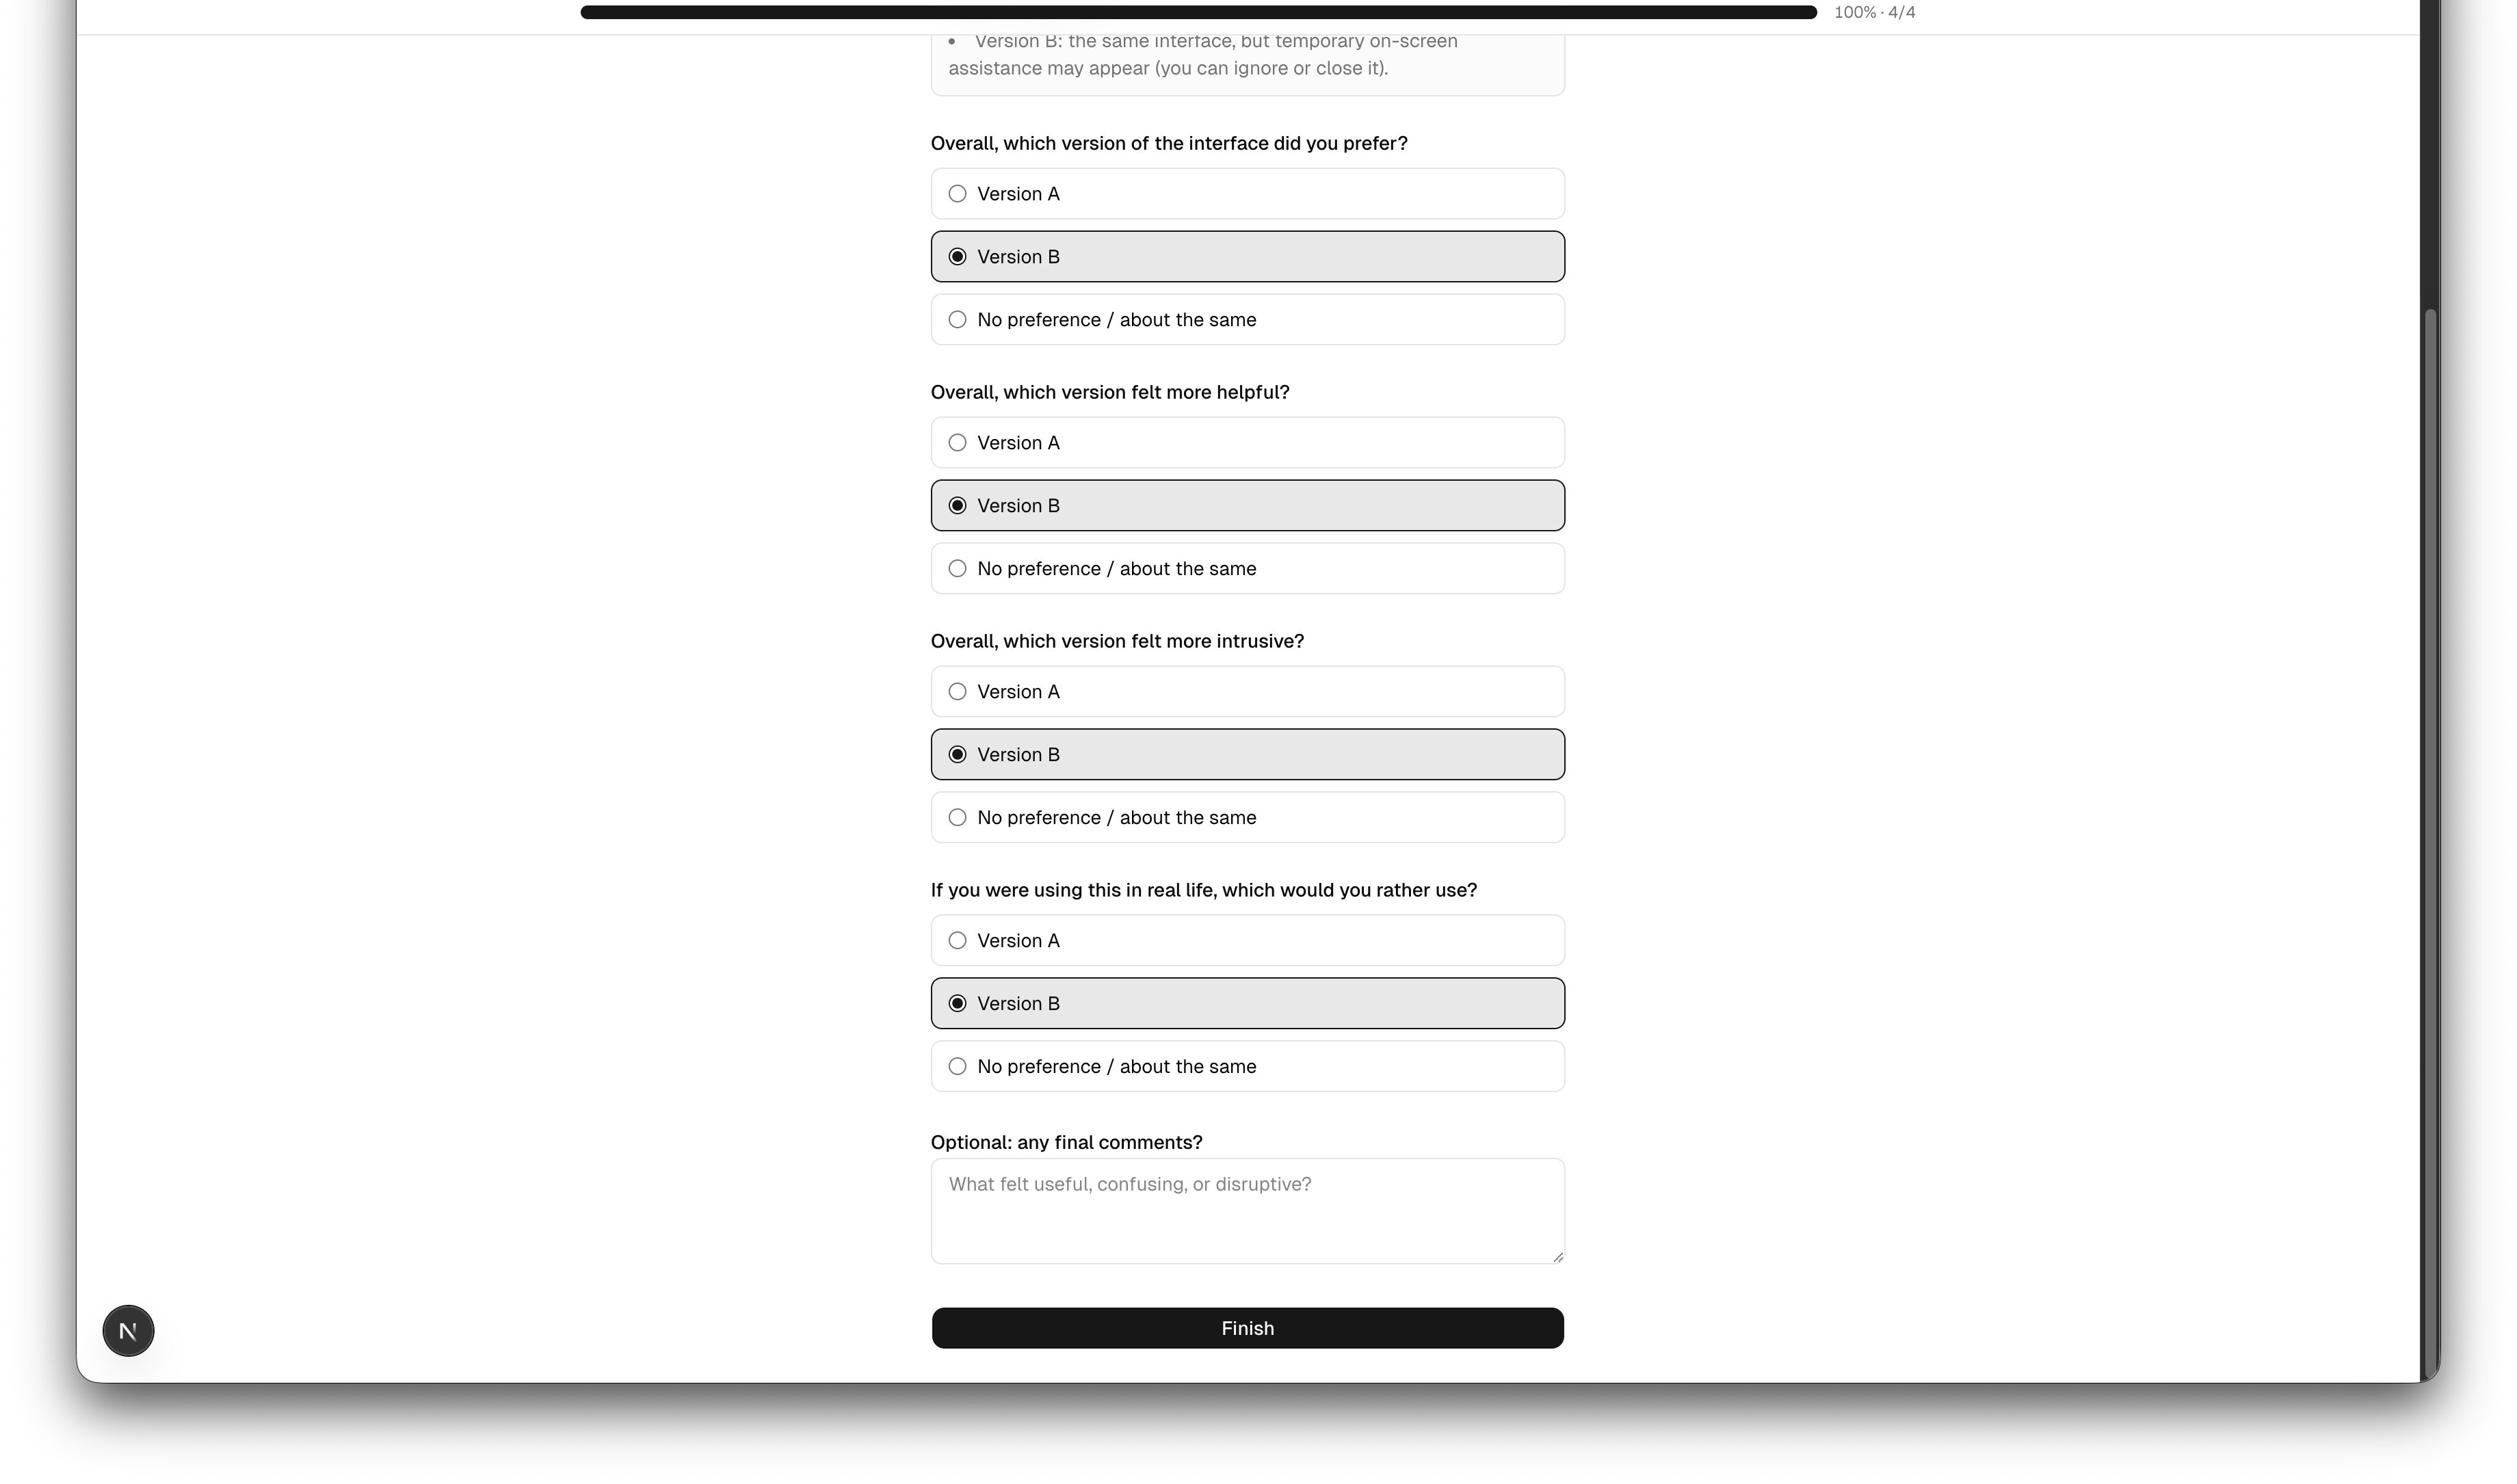
\includegraphics[width=\textwidth]{graphics/example-flow-11.png}
        \caption{Completed final questionnaire with comparative judgments recorded.}
    \end{subfigure}
    \caption{Participant-flow walkthrough, part~5: final comparison questions at the end of the session.}
    \label{fig:appendix-flow-5}
\end{figure}

\subsection{Interpretive Note}

These listings are sufficient to show the main route from raw study records to reported results: first the valid sample was defined consistently, then paired statistical tests were run, then publication-quality figures were generated, and finally the resulting numerical outputs were written into LaTeX commands consumed by the manuscript itself. This is the core evidence needed to demonstrate that the quantitative results chapter was generated through a reproducible analysis workflow rather than through manual transcription.

\end{appendices}
